% Options for packages loaded elsewhere
\PassOptionsToPackage{unicode}{hyperref}
\PassOptionsToPackage{hyphens}{url}
%
\documentclass[
  11pt,
]{article}
\usepackage{amsmath,amssymb}
\usepackage{lmodern}
\usepackage{ifxetex,ifluatex}
\ifnum 0\ifxetex 1\fi\ifluatex 1\fi=0 % if pdftex
  \usepackage[T1]{fontenc}
  \usepackage[utf8]{inputenc}
  \usepackage{textcomp} % provide euro and other symbols
\else % if luatex or xetex
  \usepackage{unicode-math}
  \defaultfontfeatures{Scale=MatchLowercase}
  \defaultfontfeatures[\rmfamily]{Ligatures=TeX,Scale=1}
\fi
% Use upquote if available, for straight quotes in verbatim environments
\IfFileExists{upquote.sty}{\usepackage{upquote}}{}
\IfFileExists{microtype.sty}{% use microtype if available
  \usepackage[]{microtype}
  \UseMicrotypeSet[protrusion]{basicmath} % disable protrusion for tt fonts
}{}
\makeatletter
\@ifundefined{KOMAClassName}{% if non-KOMA class
  \IfFileExists{parskip.sty}{%
    \usepackage{parskip}
  }{% else
    \setlength{\parindent}{0pt}
    \setlength{\parskip}{6pt plus 2pt minus 1pt}}
}{% if KOMA class
  \KOMAoptions{parskip=half}}
\makeatother
\usepackage{xcolor}
\IfFileExists{xurl.sty}{\usepackage{xurl}}{} % add URL line breaks if available
\IfFileExists{bookmark.sty}{\usepackage{bookmark}}{\usepackage{hyperref}}
\hypersetup{
  pdftitle={BIST8130 - Final Proejct Codings},
  hidelinks,
  pdfcreator={LaTeX via pandoc}}
\urlstyle{same} % disable monospaced font for URLs
\usepackage[margin=1in]{geometry}
\usepackage{color}
\usepackage{fancyvrb}
\newcommand{\VerbBar}{|}
\newcommand{\VERB}{\Verb[commandchars=\\\{\}]}
\DefineVerbatimEnvironment{Highlighting}{Verbatim}{commandchars=\\\{\}}
% Add ',fontsize=\small' for more characters per line
\usepackage{framed}
\definecolor{shadecolor}{RGB}{248,248,248}
\newenvironment{Shaded}{\begin{snugshade}}{\end{snugshade}}
\newcommand{\AlertTok}[1]{\textcolor[rgb]{0.94,0.16,0.16}{#1}}
\newcommand{\AnnotationTok}[1]{\textcolor[rgb]{0.56,0.35,0.01}{\textbf{\textit{#1}}}}
\newcommand{\AttributeTok}[1]{\textcolor[rgb]{0.77,0.63,0.00}{#1}}
\newcommand{\BaseNTok}[1]{\textcolor[rgb]{0.00,0.00,0.81}{#1}}
\newcommand{\BuiltInTok}[1]{#1}
\newcommand{\CharTok}[1]{\textcolor[rgb]{0.31,0.60,0.02}{#1}}
\newcommand{\CommentTok}[1]{\textcolor[rgb]{0.56,0.35,0.01}{\textit{#1}}}
\newcommand{\CommentVarTok}[1]{\textcolor[rgb]{0.56,0.35,0.01}{\textbf{\textit{#1}}}}
\newcommand{\ConstantTok}[1]{\textcolor[rgb]{0.00,0.00,0.00}{#1}}
\newcommand{\ControlFlowTok}[1]{\textcolor[rgb]{0.13,0.29,0.53}{\textbf{#1}}}
\newcommand{\DataTypeTok}[1]{\textcolor[rgb]{0.13,0.29,0.53}{#1}}
\newcommand{\DecValTok}[1]{\textcolor[rgb]{0.00,0.00,0.81}{#1}}
\newcommand{\DocumentationTok}[1]{\textcolor[rgb]{0.56,0.35,0.01}{\textbf{\textit{#1}}}}
\newcommand{\ErrorTok}[1]{\textcolor[rgb]{0.64,0.00,0.00}{\textbf{#1}}}
\newcommand{\ExtensionTok}[1]{#1}
\newcommand{\FloatTok}[1]{\textcolor[rgb]{0.00,0.00,0.81}{#1}}
\newcommand{\FunctionTok}[1]{\textcolor[rgb]{0.00,0.00,0.00}{#1}}
\newcommand{\ImportTok}[1]{#1}
\newcommand{\InformationTok}[1]{\textcolor[rgb]{0.56,0.35,0.01}{\textbf{\textit{#1}}}}
\newcommand{\KeywordTok}[1]{\textcolor[rgb]{0.13,0.29,0.53}{\textbf{#1}}}
\newcommand{\NormalTok}[1]{#1}
\newcommand{\OperatorTok}[1]{\textcolor[rgb]{0.81,0.36,0.00}{\textbf{#1}}}
\newcommand{\OtherTok}[1]{\textcolor[rgb]{0.56,0.35,0.01}{#1}}
\newcommand{\PreprocessorTok}[1]{\textcolor[rgb]{0.56,0.35,0.01}{\textit{#1}}}
\newcommand{\RegionMarkerTok}[1]{#1}
\newcommand{\SpecialCharTok}[1]{\textcolor[rgb]{0.00,0.00,0.00}{#1}}
\newcommand{\SpecialStringTok}[1]{\textcolor[rgb]{0.31,0.60,0.02}{#1}}
\newcommand{\StringTok}[1]{\textcolor[rgb]{0.31,0.60,0.02}{#1}}
\newcommand{\VariableTok}[1]{\textcolor[rgb]{0.00,0.00,0.00}{#1}}
\newcommand{\VerbatimStringTok}[1]{\textcolor[rgb]{0.31,0.60,0.02}{#1}}
\newcommand{\WarningTok}[1]{\textcolor[rgb]{0.56,0.35,0.01}{\textbf{\textit{#1}}}}
\usepackage{longtable,booktabs,array}
\usepackage{calc} % for calculating minipage widths
% Correct order of tables after \paragraph or \subparagraph
\usepackage{etoolbox}
\makeatletter
\patchcmd\longtable{\par}{\if@noskipsec\mbox{}\fi\par}{}{}
\makeatother
% Allow footnotes in longtable head/foot
\IfFileExists{footnotehyper.sty}{\usepackage{footnotehyper}}{\usepackage{footnote}}
\makesavenoteenv{longtable}
\usepackage{graphicx}
\makeatletter
\def\maxwidth{\ifdim\Gin@nat@width>\linewidth\linewidth\else\Gin@nat@width\fi}
\def\maxheight{\ifdim\Gin@nat@height>\textheight\textheight\else\Gin@nat@height\fi}
\makeatother
% Scale images if necessary, so that they will not overflow the page
% margins by default, and it is still possible to overwrite the defaults
% using explicit options in \includegraphics[width, height, ...]{}
\setkeys{Gin}{width=\maxwidth,height=\maxheight,keepaspectratio}
% Set default figure placement to htbp
\makeatletter
\def\fps@figure{htbp}
\makeatother
\setlength{\emergencystretch}{3em} % prevent overfull lines
\providecommand{\tightlist}{%
  \setlength{\itemsep}{0pt}\setlength{\parskip}{0pt}}
\setcounter{secnumdepth}{-\maxdimen} % remove section numbering
\ifluatex
  \usepackage{selnolig}  % disable illegal ligatures
\fi

\title{BIST8130 - Final Proejct Codings}
\author{}
\date{\vspace{-2.5em}11/22/2021}

\begin{document}
\maketitle

\begin{Shaded}
\begin{Highlighting}[]
\FunctionTok{library}\NormalTok{(tidyverse)}
\FunctionTok{library}\NormalTok{(corrplot)}
\FunctionTok{library}\NormalTok{(leaps)}
\FunctionTok{library}\NormalTok{(performance)}
\FunctionTok{library}\NormalTok{(MASS)}
\FunctionTok{library}\NormalTok{(caret)}

\NormalTok{knitr}\SpecialCharTok{::}\NormalTok{opts\_chunk}\SpecialCharTok{$}\FunctionTok{set}\NormalTok{(}
  \AttributeTok{fig.width =} \DecValTok{8}\NormalTok{,}
  \AttributeTok{fig.asp =}\NormalTok{ .}\DecValTok{6}\NormalTok{,}
  \AttributeTok{out.width =} \StringTok{"90\%"}\NormalTok{,}
  \AttributeTok{echo =} \ConstantTok{TRUE}\NormalTok{, }\AttributeTok{warning =} \ConstantTok{FALSE}\NormalTok{, }\AttributeTok{dpi=}\DecValTok{300}
  
\NormalTok{)}
\end{Highlighting}
\end{Shaded}

\hypertarget{step-1-data-preprocessing}{%
\subsection{Step 1: Data
Preprocessing}\label{step-1-data-preprocessing}}

After importing the csv file containing the County Demographic
Information (CDI) data, we notice that crimes, physicians, and hospital
beds are given as numbers, while other info are given as proportions. We
therefore compute the number of crimes, physicians, and hospital beds
per 1000 people.

\begin{Shaded}
\begin{Highlighting}[]
\NormalTok{cdi\_data }\OtherTok{=} \FunctionTok{read\_csv}\NormalTok{(}\StringTok{"./data/cdi.csv"}\NormalTok{) }\SpecialCharTok{\%\textgreater{}\%}
\NormalTok{  janitor}\SpecialCharTok{::}\FunctionTok{clean\_names}\NormalTok{() }\SpecialCharTok{\%\textgreater{}\%}
  \FunctionTok{mutate}\NormalTok{(}
    \AttributeTok{cty\_state =} \FunctionTok{str\_c}\NormalTok{(cty,}\StringTok{","}\NormalTok{,state),}
    \AttributeTok{docs\_rate\_1000 =} \DecValTok{1000} \SpecialCharTok{*}\NormalTok{ docs}\SpecialCharTok{/}\NormalTok{pop, }
    \CommentTok{\# Compute number of doctors/hospital beds per 1000 people.}
    \AttributeTok{beds\_rate\_1000 =} \DecValTok{1000} \SpecialCharTok{*}\NormalTok{ beds}\SpecialCharTok{/}\NormalTok{pop,}
    \AttributeTok{density =} \FunctionTok{as.numeric}\NormalTok{(pop)}\SpecialCharTok{/}\FunctionTok{as.numeric}\NormalTok{(area),}
    \AttributeTok{crime\_rate\_1000 =} \DecValTok{1000} \SpecialCharTok{*}\NormalTok{ crimes}\SpecialCharTok{/}\NormalTok{pop) }\SpecialCharTok{\%\textgreater{}\%} 
  \CommentTok{\# Compute number of crimes per 1000 people. }
\NormalTok{  dplyr}\SpecialCharTok{::}\FunctionTok{select}\NormalTok{(}\SpecialCharTok{{-}}\NormalTok{docs,}\SpecialCharTok{{-}}\NormalTok{beds,}\SpecialCharTok{{-}}\NormalTok{crimes) }\SpecialCharTok{\%\textgreater{}\%}
  \FunctionTok{relocate}\NormalTok{(id,cty\_state,cty)}

\CommentTok{\#knitr::kable(head(cdi\_data))}
\end{Highlighting}
\end{Shaded}

\hypertarget{step-2---exploratory-analysis}{%
\subsection{Step 2 - Exploratory
Analysis}\label{step-2---exploratory-analysis}}

We then take a closer look of each variables, calculate the pairwise
correlations between variables, and list all the correlations between
the crime rate (our interest) and all other variables.

\begin{Shaded}
\begin{Highlighting}[]
\NormalTok{cdi\_data\_exp }\OtherTok{=}\NormalTok{ cdi\_data }\SpecialCharTok{\%\textgreater{}\%}
\NormalTok{  dplyr}\SpecialCharTok{::}\FunctionTok{select}\NormalTok{(}\SpecialCharTok{{-}}\NormalTok{id,}\SpecialCharTok{{-}}\NormalTok{cty,}\SpecialCharTok{{-}}\NormalTok{state, }\SpecialCharTok{{-}}\NormalTok{cty\_state) }
\end{Highlighting}
\end{Shaded}

\begin{Shaded}
\begin{Highlighting}[]
\FunctionTok{par}\NormalTok{(}\AttributeTok{mfrow=}\FunctionTok{c}\NormalTok{(}\DecValTok{4}\NormalTok{,}\DecValTok{3}\NormalTok{))}
\FunctionTok{boxplot}\NormalTok{(cdi\_data\_exp}\SpecialCharTok{$}\NormalTok{area,}\AttributeTok{main=}\StringTok{"Area"}\NormalTok{)}
\FunctionTok{boxplot}\NormalTok{(cdi\_data\_exp}\SpecialCharTok{$}\NormalTok{pop,}\AttributeTok{main=}\StringTok{"Population"}\NormalTok{)}
\FunctionTok{boxplot}\NormalTok{(cdi\_data\_exp}\SpecialCharTok{$}\NormalTok{pop18,}\AttributeTok{main=}\StringTok{"Population 18{-}34"}\NormalTok{)}
\FunctionTok{boxplot}\NormalTok{(cdi\_data\_exp}\SpecialCharTok{$}\NormalTok{pop65,}\AttributeTok{main=}\StringTok{"Population 65+"}\NormalTok{)}
\FunctionTok{boxplot}\NormalTok{(cdi\_data\_exp}\SpecialCharTok{$}\NormalTok{hsgrad,}\AttributeTok{main=}\StringTok{"Highschool grads"}\NormalTok{)}
\FunctionTok{boxplot}\NormalTok{(cdi\_data\_exp}\SpecialCharTok{$}\NormalTok{bagrad,}\AttributeTok{main=}\StringTok{"Bachelor\textquotesingle{}s grads"}\NormalTok{)}

\CommentTok{\#par(mfrow=c(2,3))}
\FunctionTok{boxplot}\NormalTok{(cdi\_data\_exp}\SpecialCharTok{$}\NormalTok{poverty,}\AttributeTok{main=}\StringTok{"Poverty Rate"}\NormalTok{)}
\FunctionTok{boxplot}\NormalTok{(cdi\_data\_exp}\SpecialCharTok{$}\NormalTok{unemp,}\AttributeTok{main=}\StringTok{"Unemployment Rate"}\NormalTok{)}
\FunctionTok{boxplot}\NormalTok{(cdi\_data\_exp}\SpecialCharTok{$}\NormalTok{pcincome,}\AttributeTok{main=}\StringTok{"Income Per Capita"}\NormalTok{)}
\FunctionTok{boxplot}\NormalTok{(cdi\_data\_exp}\SpecialCharTok{$}\NormalTok{totalinc,}\AttributeTok{main=}\StringTok{"Income Total"}\NormalTok{)}
\FunctionTok{boxplot}\NormalTok{(cdi\_data\_exp}\SpecialCharTok{$}\NormalTok{docs\_rate\_1000,}\AttributeTok{main=}\StringTok{"Active Physicians"}\NormalTok{)}
\FunctionTok{boxplot}\NormalTok{(cdi\_data\_exp}\SpecialCharTok{$}\NormalTok{beds\_rate\_1000,}\AttributeTok{main=}\StringTok{"Hospital Beds"}\NormalTok{)}
\end{Highlighting}
\end{Shaded}

\begin{figure}
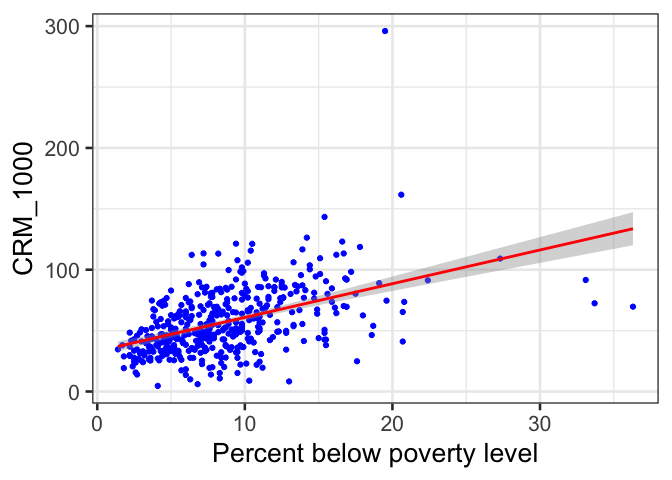
\includegraphics[width=0.9\linewidth]{main_files/figure-latex/unnamed-chunk-1-1} \caption{\label{fig:figs}boxplot of continuous variables distribution}\label{fig:unnamed-chunk-1}
\end{figure}

\begin{Shaded}
\begin{Highlighting}[]
\FunctionTok{par}\NormalTok{(}\AttributeTok{mfrow=}\FunctionTok{c}\NormalTok{(}\DecValTok{1}\NormalTok{,}\DecValTok{1}\NormalTok{))}

\FunctionTok{ggplot}\NormalTok{(cdi\_data,}\FunctionTok{aes}\NormalTok{(region)) }\SpecialCharTok{+} 
  \FunctionTok{geom\_histogram}\NormalTok{(}\AttributeTok{binwidth =} \FloatTok{0.5}\NormalTok{) }\SpecialCharTok{+}
  \FunctionTok{theme\_classic}\NormalTok{() }\SpecialCharTok{+}
  \FunctionTok{xlab}\NormalTok{(}\StringTok{"Region"}\NormalTok{)}\SpecialCharTok{+}
  \FunctionTok{ylab}\NormalTok{(}\StringTok{"Count"}\NormalTok{) }\SpecialCharTok{+}
  \FunctionTok{labs}\NormalTok{(}\AttributeTok{title =} \StringTok{"Histogram: Counts of four regions"}\NormalTok{)}
\end{Highlighting}
\end{Shaded}

\begin{figure}
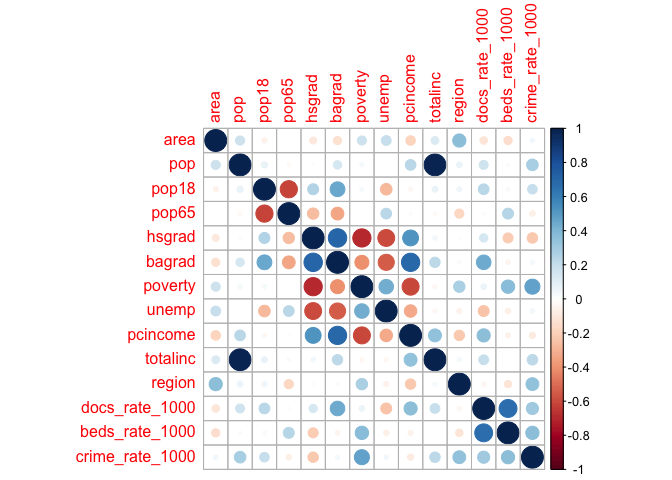
\includegraphics[width=0.9\linewidth]{main_files/figure-latex/unnamed-chunk-2-1} \caption{\label{fig:figs}Histogram of catagorical variable:region distribution}\label{fig:unnamed-chunk-2}
\end{figure}

\begin{Shaded}
\begin{Highlighting}[]
\FunctionTok{boxplot}\NormalTok{(cdi\_data\_exp}\SpecialCharTok{$}\NormalTok{crime\_rate\_1000,}\AttributeTok{main=}\StringTok{"Boxplot of Crime Rate"}\NormalTok{,}\AttributeTok{horizontal =} \ConstantTok{TRUE}\NormalTok{)}
\end{Highlighting}
\end{Shaded}

\begin{figure}
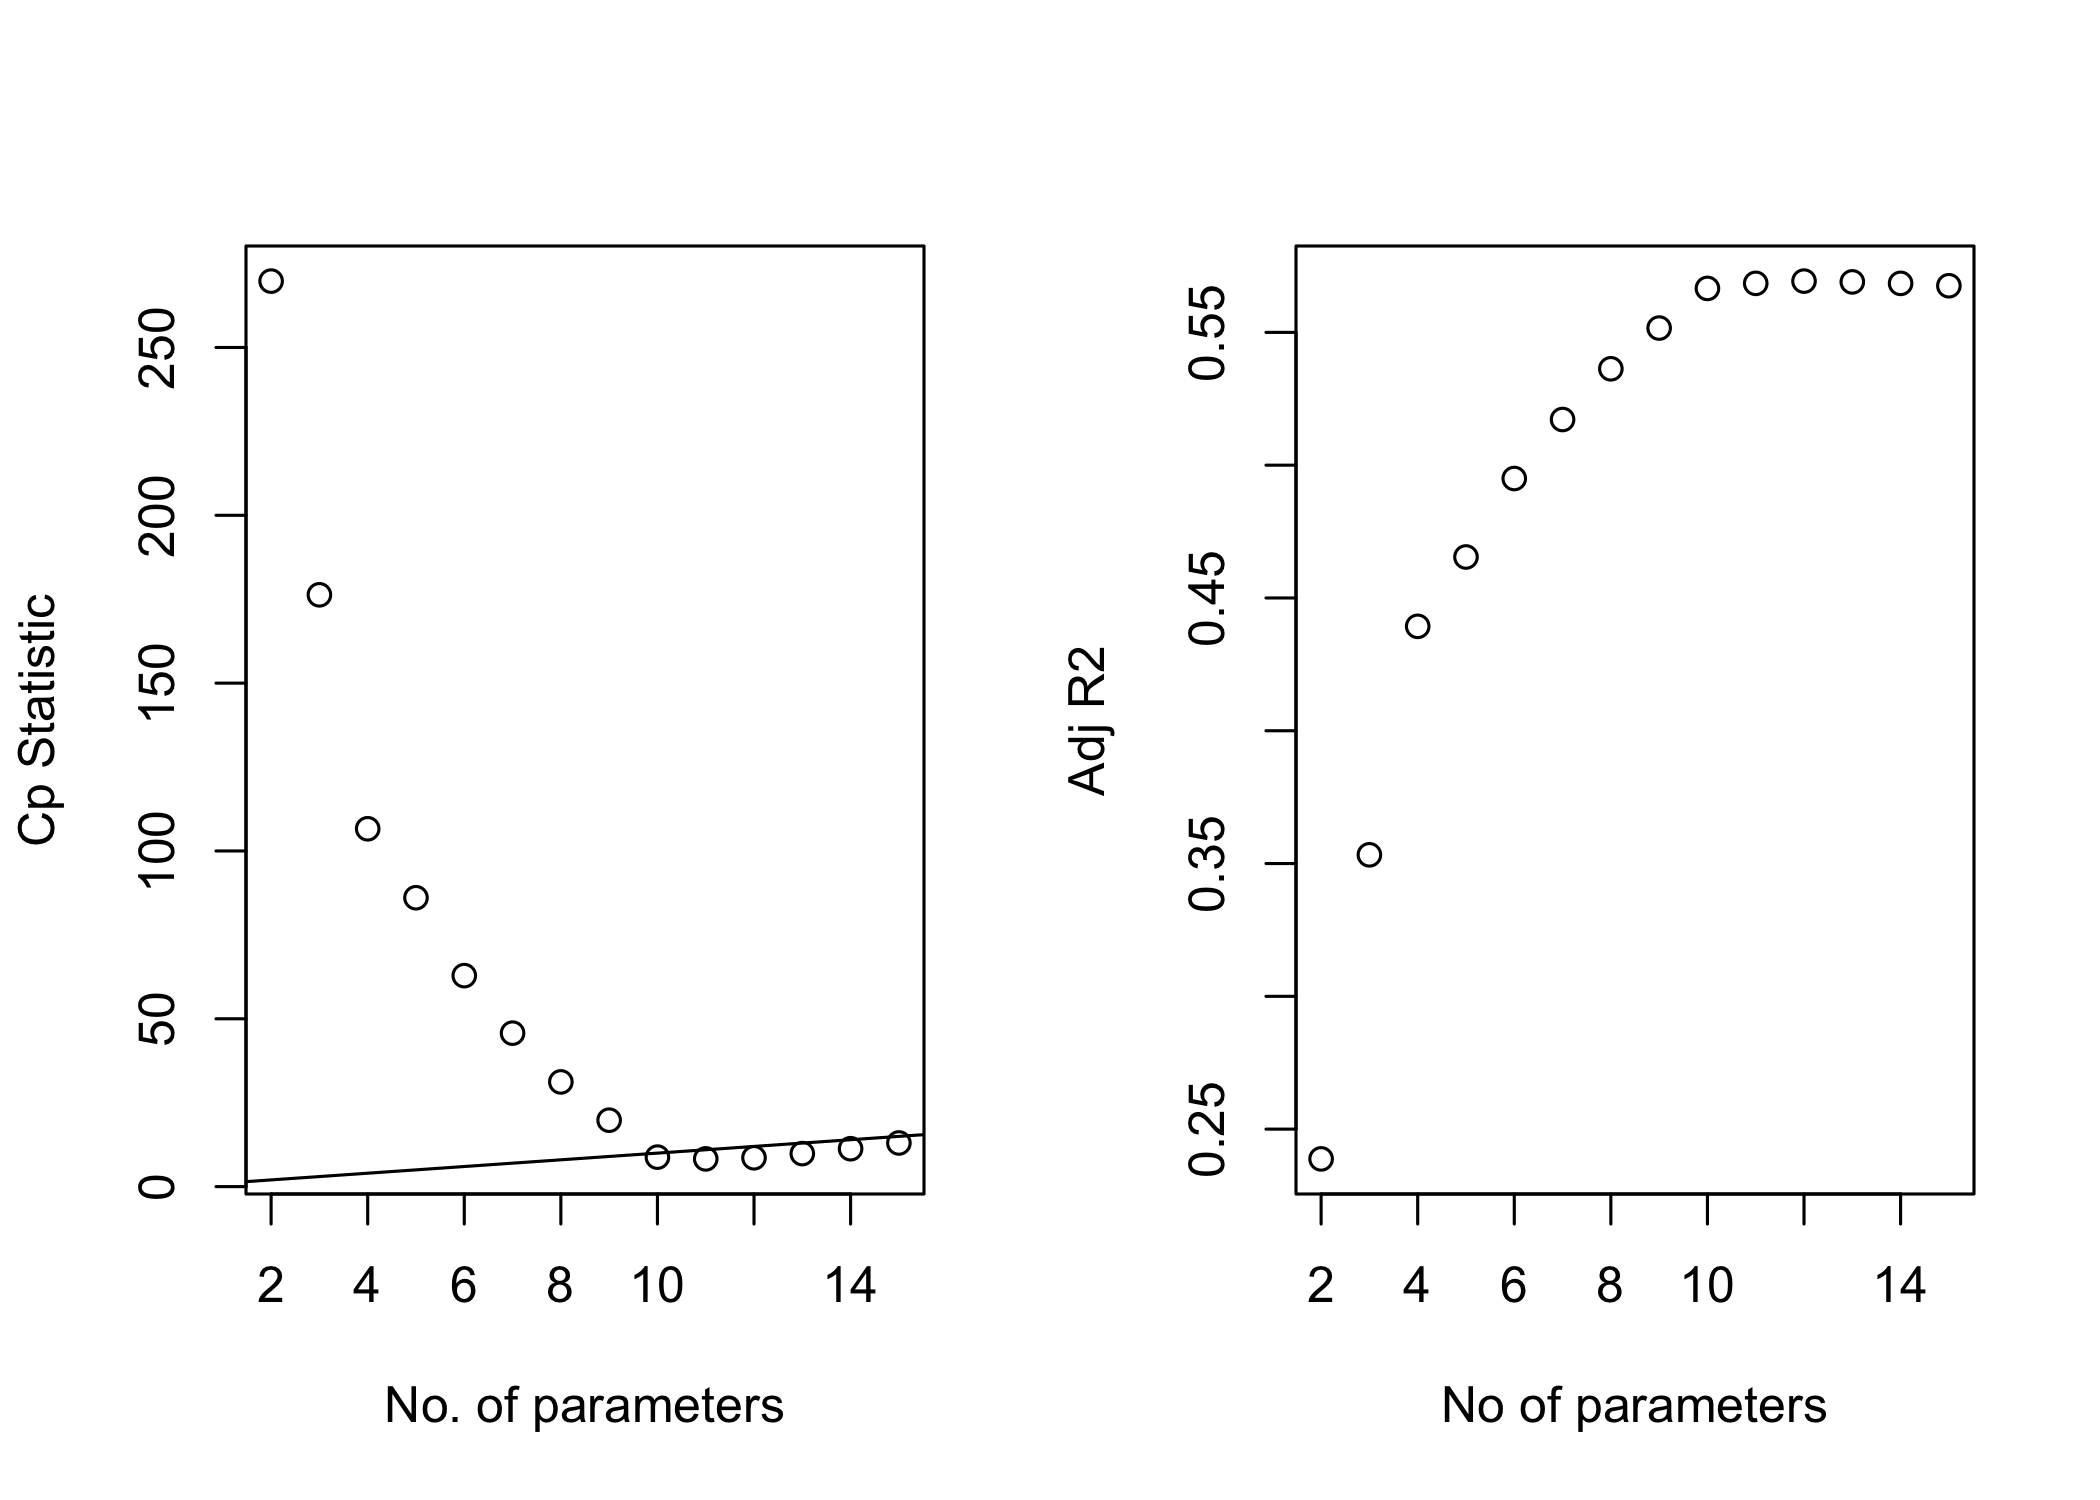
\includegraphics[width=0.9\linewidth]{main_files/figure-latex/unnamed-chunk-3-1} \caption{\label{fig:figs}boxplot of dependent variable: crime rate}\label{fig:unnamed-chunk-3}
\end{figure}

\begin{Shaded}
\begin{Highlighting}[]
\CommentTok{\# data exploratory}
\CommentTok{\# pairs(cdi\_data\_exp)}
\end{Highlighting}
\end{Shaded}

\begin{Shaded}
\begin{Highlighting}[]
\CommentTok{\# correlation plot}
\NormalTok{cdi\_data\_cor }\OtherTok{=} \FunctionTok{cor}\NormalTok{(cdi\_data\_exp)}
\FunctionTok{corrplot}\NormalTok{(cdi\_data\_cor, }\AttributeTok{type =} \StringTok{"upper"}\NormalTok{, }\AttributeTok{diag =} \ConstantTok{FALSE}\NormalTok{, }\AttributeTok{title =} \StringTok{"Correlation heatmap"}\NormalTok{)}
\end{Highlighting}
\end{Shaded}

\begin{figure}
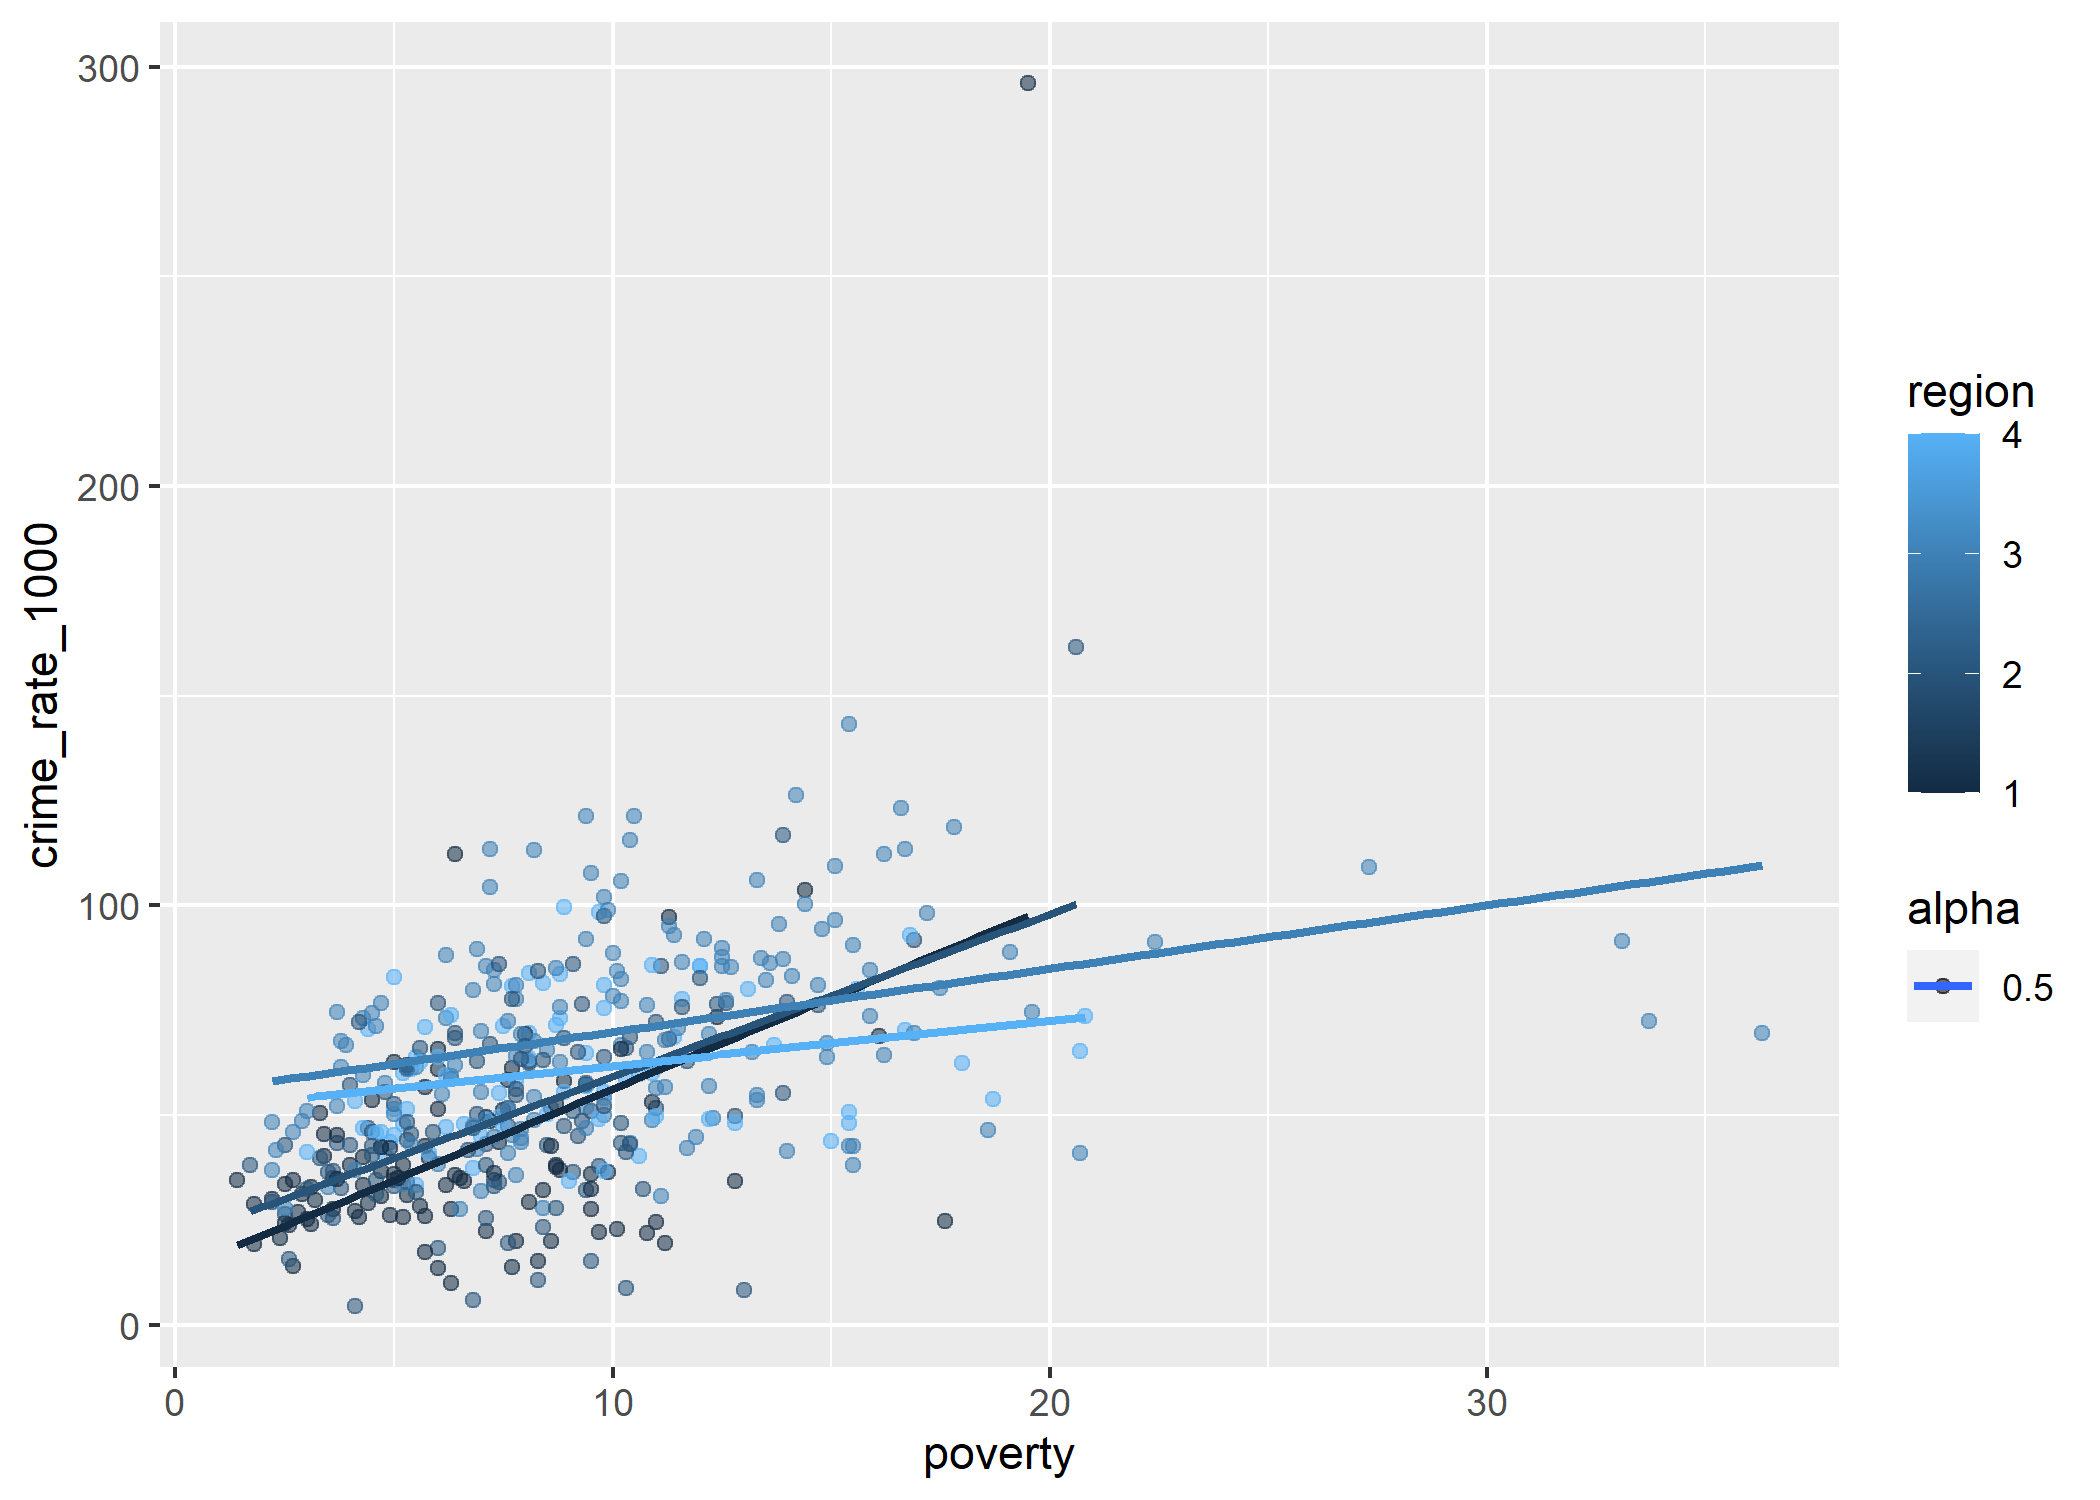
\includegraphics[width=0.9\linewidth]{main_files/figure-latex/unnamed-chunk-5-1} \caption{\label{fig:figs}Correlation heatmap}\label{fig:unnamed-chunk-5}
\end{figure}

\begin{Shaded}
\begin{Highlighting}[]
\NormalTok{crime\_1000\_cor }\OtherTok{=} \FunctionTok{data.frame}\NormalTok{(cdi\_data\_cor) }\SpecialCharTok{\%\textgreater{}\%} 
\NormalTok{  dplyr}\SpecialCharTok{::}\FunctionTok{select}\NormalTok{(}\StringTok{"Crime Rate (Per 1000)"} \OtherTok{=}\NormalTok{ crime\_rate\_1000) }\SpecialCharTok{\%\textgreater{}\%} 
  \FunctionTok{t}\NormalTok{()}

\CommentTok{\#knitr::kable(crime\_1000\_cor,digits = 2) }
\end{Highlighting}
\end{Shaded}

\hypertarget{trainingtest-set-split}{%
\subsection{Training/Test set split}\label{trainingtest-set-split}}

\begin{Shaded}
\begin{Highlighting}[]
\NormalTok{cdi\_data }\OtherTok{=}\NormalTok{ cdi\_data }\SpecialCharTok{\%\textgreater{}\%} 
\NormalTok{  dplyr}\SpecialCharTok{::}\FunctionTok{select}\NormalTok{(}\SpecialCharTok{{-}}\NormalTok{id,}\SpecialCharTok{{-}}\NormalTok{cty\_state, }\SpecialCharTok{{-}}\NormalTok{cty,}\SpecialCharTok{{-}}\NormalTok{state) }\SpecialCharTok{\%\textgreater{}\%} 
  \FunctionTok{mutate}\NormalTok{(}\AttributeTok{region =} \FunctionTok{factor}\NormalTok{(region))}

\FunctionTok{set.seed}\NormalTok{(}\DecValTok{1}\NormalTok{)}
\NormalTok{dt }\OtherTok{=} \FunctionTok{sort}\NormalTok{(}\FunctionTok{sample}\NormalTok{(}\FunctionTok{nrow}\NormalTok{(cdi\_data), }\FunctionTok{nrow}\NormalTok{(cdi\_data)}\SpecialCharTok{*}\NormalTok{.}\DecValTok{9}\NormalTok{))}
\NormalTok{train\_data }\OtherTok{=}\NormalTok{ cdi\_data[dt,]}
\NormalTok{test\_data }\OtherTok{=}\NormalTok{ cdi\_data[}\SpecialCharTok{{-}}\NormalTok{dt,]}
\end{Highlighting}
\end{Shaded}

\hypertarget{remove-outliers-and-high-leverage-point}{%
\subsection{Remove outliers and high leverage
point}\label{remove-outliers-and-high-leverage-point}}

\begin{Shaded}
\begin{Highlighting}[]
\CommentTok{\# Remove high leverage points}

\NormalTok{cdi\_data\_clean }\OtherTok{=}\NormalTok{ train\_data[train\_data}\SpecialCharTok{$}\NormalTok{area }\SpecialCharTok{\textgreater{}=} \FunctionTok{quantile}\NormalTok{(train\_data}\SpecialCharTok{$}\NormalTok{area,}\FloatTok{0.002}\NormalTok{) }\SpecialCharTok{\&}\NormalTok{ train\_data}\SpecialCharTok{$}\NormalTok{area }\SpecialCharTok{\textless{}=} \FunctionTok{quantile}\NormalTok{(train\_data}\SpecialCharTok{$}\NormalTok{area,}\FloatTok{0.998}\NormalTok{),]}
\NormalTok{cdi\_data\_clean }\OtherTok{=}\NormalTok{ cdi\_data\_clean[cdi\_data\_clean}\SpecialCharTok{$}\NormalTok{pop }\SpecialCharTok{\textgreater{}=} \FunctionTok{quantile}\NormalTok{(cdi\_data\_clean}\SpecialCharTok{$}\NormalTok{pop,}\FloatTok{0.002}\NormalTok{) }\SpecialCharTok{\&}\NormalTok{ cdi\_data\_clean}\SpecialCharTok{$}\NormalTok{pop }\SpecialCharTok{\textless{}=} \FunctionTok{quantile}\NormalTok{(cdi\_data\_clean}\SpecialCharTok{$}\NormalTok{pop,}\FloatTok{0.998}\NormalTok{),]}
\NormalTok{cdi\_data\_clean }\OtherTok{=}\NormalTok{ cdi\_data\_clean[cdi\_data\_clean}\SpecialCharTok{$}\NormalTok{pop18 }\SpecialCharTok{\textgreater{}=} \FunctionTok{quantile}\NormalTok{(cdi\_data\_clean}\SpecialCharTok{$}\NormalTok{pop18,}\FloatTok{0.002}\NormalTok{) }\SpecialCharTok{\&}\NormalTok{ cdi\_data\_clean}\SpecialCharTok{$}\NormalTok{pop18 }\SpecialCharTok{\textless{}=} \FunctionTok{quantile}\NormalTok{(cdi\_data\_clean}\SpecialCharTok{$}\NormalTok{pop18,}\FloatTok{0.998}\NormalTok{),]}
\NormalTok{cdi\_data\_clean }\OtherTok{=}\NormalTok{ cdi\_data\_clean[cdi\_data\_clean}\SpecialCharTok{$}\NormalTok{pop65 }\SpecialCharTok{\textgreater{}=} \FunctionTok{quantile}\NormalTok{(cdi\_data\_clean}\SpecialCharTok{$}\NormalTok{pop65,}\FloatTok{0.002}\NormalTok{) }\SpecialCharTok{\&}\NormalTok{ cdi\_data\_clean}\SpecialCharTok{$}\NormalTok{pop65 }\SpecialCharTok{\textless{}=} \FunctionTok{quantile}\NormalTok{(cdi\_data\_clean}\SpecialCharTok{$}\NormalTok{pop65,}\FloatTok{0.998}\NormalTok{),]}
\NormalTok{cdi\_data\_clean }\OtherTok{=}\NormalTok{ cdi\_data\_clean[cdi\_data\_clean}\SpecialCharTok{$}\NormalTok{hsgrad }\SpecialCharTok{\textgreater{}=} \FunctionTok{quantile}\NormalTok{(cdi\_data\_clean}\SpecialCharTok{$}\NormalTok{hsgrad,}\FloatTok{0.002}\NormalTok{) }\SpecialCharTok{\&}\NormalTok{ cdi\_data\_clean}\SpecialCharTok{$}\NormalTok{hsgrad }\SpecialCharTok{\textless{}=} \FunctionTok{quantile}\NormalTok{(cdi\_data\_clean}\SpecialCharTok{$}\NormalTok{hsgrad,}\FloatTok{0.998}\NormalTok{),]}
\NormalTok{cdi\_data\_clean }\OtherTok{=}\NormalTok{ cdi\_data\_clean[cdi\_data\_clean}\SpecialCharTok{$}\NormalTok{bagrad }\SpecialCharTok{\textgreater{}=} \FunctionTok{quantile}\NormalTok{(cdi\_data\_clean}\SpecialCharTok{$}\NormalTok{bagrad,}\FloatTok{0.002}\NormalTok{) }\SpecialCharTok{\&}\NormalTok{ cdi\_data\_clean}\SpecialCharTok{$}\NormalTok{bagrad }\SpecialCharTok{\textless{}=} \FunctionTok{quantile}\NormalTok{(cdi\_data\_clean}\SpecialCharTok{$}\NormalTok{bagrad,}\FloatTok{0.998}\NormalTok{),]}

\NormalTok{cdi\_data\_clean }\OtherTok{=}\NormalTok{ cdi\_data\_clean[cdi\_data\_clean}\SpecialCharTok{$}\NormalTok{poverty }\SpecialCharTok{\textgreater{}=} \FunctionTok{quantile}\NormalTok{(cdi\_data\_clean}\SpecialCharTok{$}\NormalTok{poverty,}\FloatTok{0.002}\NormalTok{) }\SpecialCharTok{\&}\NormalTok{ cdi\_data\_clean}\SpecialCharTok{$}\NormalTok{poverty }\SpecialCharTok{\textless{}=} \FunctionTok{quantile}\NormalTok{(cdi\_data\_clean}\SpecialCharTok{$}\NormalTok{poverty,}\FloatTok{0.998}\NormalTok{),]}
\NormalTok{cdi\_data\_clean }\OtherTok{=}\NormalTok{ cdi\_data\_clean[cdi\_data\_clean}\SpecialCharTok{$}\NormalTok{unemp }\SpecialCharTok{\textgreater{}=} \FunctionTok{quantile}\NormalTok{(cdi\_data\_clean}\SpecialCharTok{$}\NormalTok{unemp,}\FloatTok{0.002}\NormalTok{) }\SpecialCharTok{\&}\NormalTok{ cdi\_data\_clean}\SpecialCharTok{$}\NormalTok{unemp }\SpecialCharTok{\textless{}=} \FunctionTok{quantile}\NormalTok{(cdi\_data\_clean}\SpecialCharTok{$}\NormalTok{unemp,}\FloatTok{0.998}\NormalTok{),]}
\NormalTok{cdi\_data\_clean }\OtherTok{=}\NormalTok{ cdi\_data\_clean[cdi\_data\_clean}\SpecialCharTok{$}\NormalTok{pcincome }\SpecialCharTok{\textgreater{}=} \FunctionTok{quantile}\NormalTok{(cdi\_data\_clean}\SpecialCharTok{$}\NormalTok{pcincome,}\FloatTok{0.002}\NormalTok{) }\SpecialCharTok{\&}\NormalTok{ cdi\_data\_clean}\SpecialCharTok{$}\NormalTok{pcincome }\SpecialCharTok{\textless{}=} \FunctionTok{quantile}\NormalTok{(cdi\_data\_clean}\SpecialCharTok{$}\NormalTok{pcincome,}\FloatTok{0.998}\NormalTok{),]}
\NormalTok{cdi\_data\_clean }\OtherTok{=}\NormalTok{ cdi\_data\_clean[cdi\_data\_clean}\SpecialCharTok{$}\NormalTok{totalinc }\SpecialCharTok{\textgreater{}=} \FunctionTok{quantile}\NormalTok{(cdi\_data\_clean}\SpecialCharTok{$}\NormalTok{totalinc,}\FloatTok{0.002}\NormalTok{) }\SpecialCharTok{\&}\NormalTok{ cdi\_data\_clean}\SpecialCharTok{$}\NormalTok{totalinc }\SpecialCharTok{\textless{}=} \FunctionTok{quantile}\NormalTok{(cdi\_data\_clean}\SpecialCharTok{$}\NormalTok{totalinc,}\FloatTok{0.998}\NormalTok{),]}
\NormalTok{cdi\_data\_clean }\OtherTok{=}\NormalTok{ cdi\_data\_clean[cdi\_data\_clean}\SpecialCharTok{$}\NormalTok{docs\_rate\_1000 }\SpecialCharTok{\textgreater{}=} \FunctionTok{quantile}\NormalTok{(cdi\_data\_clean}\SpecialCharTok{$}\NormalTok{docs\_rate\_1000,}\FloatTok{0.002}\NormalTok{) }\SpecialCharTok{\&}\NormalTok{ cdi\_data\_clean}\SpecialCharTok{$}\NormalTok{docs\_rate\_1000 }\SpecialCharTok{\textless{}=} \FunctionTok{quantile}\NormalTok{(cdi\_data\_clean}\SpecialCharTok{$}\NormalTok{docs\_rate\_1000,}\FloatTok{0.998}\NormalTok{),]}
\NormalTok{cdi\_data\_clean }\OtherTok{=}\NormalTok{ cdi\_data\_clean[cdi\_data\_clean}\SpecialCharTok{$}\NormalTok{beds\_rate\_1000 }\SpecialCharTok{\textgreater{}=} \FunctionTok{quantile}\NormalTok{(cdi\_data\_clean}\SpecialCharTok{$}\NormalTok{beds\_rate\_1000,}\FloatTok{0.002}\NormalTok{) }\SpecialCharTok{\&}\NormalTok{ cdi\_data\_clean}\SpecialCharTok{$}\NormalTok{beds\_rate\_1000 }\SpecialCharTok{\textless{}=} \FunctionTok{quantile}\NormalTok{(cdi\_data\_clean}\SpecialCharTok{$}\NormalTok{beds\_rate\_1000,}\FloatTok{0.998}\NormalTok{),]}
\NormalTok{cdi\_data\_clean }\OtherTok{=}\NormalTok{ cdi\_data\_clean[cdi\_data\_clean}\SpecialCharTok{$}\NormalTok{beds\_rate\_1000 }\SpecialCharTok{\textgreater{}=} \FunctionTok{quantile}\NormalTok{(cdi\_data\_clean}\SpecialCharTok{$}\NormalTok{beds\_rate\_1000,}\FloatTok{0.002}\NormalTok{) }\SpecialCharTok{\&}\NormalTok{ cdi\_data\_clean}\SpecialCharTok{$}\NormalTok{beds\_rate\_1000 }\SpecialCharTok{\textless{}=} \FunctionTok{quantile}\NormalTok{(cdi\_data\_clean}\SpecialCharTok{$}\NormalTok{beds\_rate\_1000,}\FloatTok{0.998}\NormalTok{),]}
\NormalTok{cdi\_data\_clean }\OtherTok{=}\NormalTok{ cdi\_data\_clean[cdi\_data\_clean}\SpecialCharTok{$}\NormalTok{density }\SpecialCharTok{\textgreater{}=} \FunctionTok{quantile}\NormalTok{(cdi\_data\_clean}\SpecialCharTok{$}\NormalTok{density,}\FloatTok{0.002}\NormalTok{) }\SpecialCharTok{\&}\NormalTok{ cdi\_data\_clean}\SpecialCharTok{$}\NormalTok{density }\SpecialCharTok{\textless{}=} \FunctionTok{quantile}\NormalTok{(cdi\_data\_clean}\SpecialCharTok{$}\NormalTok{density,}\FloatTok{0.998}\NormalTok{),]}

\NormalTok{cdi\_data\_clean }\OtherTok{=}\NormalTok{ cdi\_data\_clean[cdi\_data\_clean}\SpecialCharTok{$}\NormalTok{crime\_rate\_1000 }\SpecialCharTok{\textgreater{}=} \FunctionTok{quantile}\NormalTok{(cdi\_data\_clean}\SpecialCharTok{$}\NormalTok{crime\_rate\_1000,}\FloatTok{0.002}\NormalTok{) }\SpecialCharTok{\&}\NormalTok{ cdi\_data\_clean}\SpecialCharTok{$}\NormalTok{beds\_rate\_1000 }\SpecialCharTok{\textless{}=} \FunctionTok{quantile}\NormalTok{(cdi\_data\_clean}\SpecialCharTok{$}\NormalTok{crime\_rate\_1000,}\FloatTok{0.998}\NormalTok{),]}
\end{Highlighting}
\end{Shaded}

\begin{Shaded}
\begin{Highlighting}[]
\FunctionTok{par}\NormalTok{(}\AttributeTok{mfrow=}\FunctionTok{c}\NormalTok{(}\DecValTok{4}\NormalTok{,}\DecValTok{3}\NormalTok{))}
\FunctionTok{boxplot}\NormalTok{(cdi\_data\_clean}\SpecialCharTok{$}\NormalTok{area,}\AttributeTok{main=}\StringTok{"Area"}\NormalTok{)}
\FunctionTok{boxplot}\NormalTok{(cdi\_data\_clean}\SpecialCharTok{$}\NormalTok{pop,}\AttributeTok{main=}\StringTok{"Population"}\NormalTok{)}
\FunctionTok{boxplot}\NormalTok{(cdi\_data\_clean}\SpecialCharTok{$}\NormalTok{pop18,}\AttributeTok{main=}\StringTok{"Population 18{-}34"}\NormalTok{)}
\FunctionTok{boxplot}\NormalTok{(cdi\_data\_clean}\SpecialCharTok{$}\NormalTok{pop65,}\AttributeTok{main=}\StringTok{"Population 65+"}\NormalTok{)}
\FunctionTok{boxplot}\NormalTok{(cdi\_data\_clean}\SpecialCharTok{$}\NormalTok{hsgrad,}\AttributeTok{main=}\StringTok{"Highschool grads"}\NormalTok{)}
\FunctionTok{boxplot}\NormalTok{(cdi\_data\_clean}\SpecialCharTok{$}\NormalTok{bagrad,}\AttributeTok{main=}\StringTok{"Bachelor\textquotesingle{}s grads"}\NormalTok{)}

\FunctionTok{boxplot}\NormalTok{(cdi\_data\_clean}\SpecialCharTok{$}\NormalTok{poverty,}\AttributeTok{main=}\StringTok{"Poverty Rate"}\NormalTok{)}
\FunctionTok{boxplot}\NormalTok{(cdi\_data\_clean}\SpecialCharTok{$}\NormalTok{unemp,}\AttributeTok{main=}\StringTok{"Unemployment Rate"}\NormalTok{)}
\FunctionTok{boxplot}\NormalTok{(cdi\_data\_clean}\SpecialCharTok{$}\NormalTok{pcincome,}\AttributeTok{main=}\StringTok{"Income Per Capita"}\NormalTok{)}
\FunctionTok{boxplot}\NormalTok{(cdi\_data\_clean}\SpecialCharTok{$}\NormalTok{totalinc,}\AttributeTok{main=}\StringTok{"Income Total"}\NormalTok{)}
\FunctionTok{boxplot}\NormalTok{(cdi\_data\_clean}\SpecialCharTok{$}\NormalTok{docs\_rate\_1000,}\AttributeTok{main=}\StringTok{"Active Physicians"}\NormalTok{)}
\FunctionTok{boxplot}\NormalTok{(cdi\_data\_clean}\SpecialCharTok{$}\NormalTok{beds\_rate\_1000,}\AttributeTok{main=}\StringTok{"Hospital Beds"}\NormalTok{)}
\end{Highlighting}
\end{Shaded}

\begin{figure}
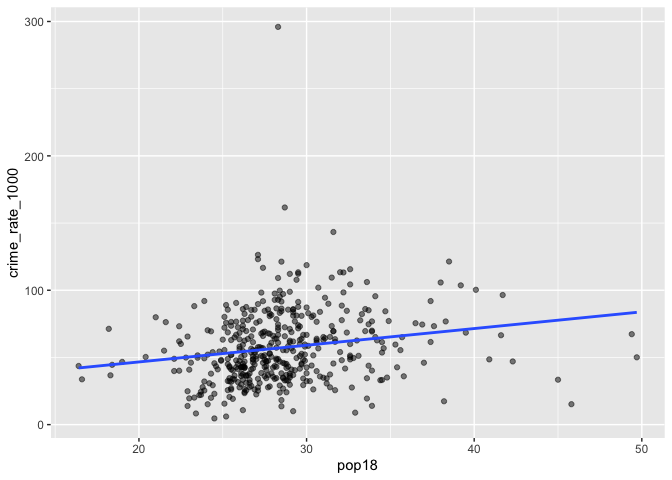
\includegraphics[width=0.9\linewidth]{main_files/figure-latex/unnamed-chunk-9-1} \caption{\label{fig:figs}Boxplot of each continuous variables aftern cleaning outliers}\label{fig:unnamed-chunk-9}
\end{figure}

\hypertarget{model-construction}{%
\subsection{Model construction}\label{model-construction}}

Data used for building model:

\begin{Shaded}
\begin{Highlighting}[]
\NormalTok{cdi\_model }\OtherTok{=}\NormalTok{ cdi\_data\_clean}
\end{Highlighting}
\end{Shaded}

\hypertarget{stepwise-regression}{%
\subsubsection{Stepwise regression}\label{stepwise-regression}}

\begin{Shaded}
\begin{Highlighting}[]
\NormalTok{full.fit }\OtherTok{=} \FunctionTok{lm}\NormalTok{(crime\_rate\_1000 }\SpecialCharTok{\textasciitilde{}}\NormalTok{ ., }\AttributeTok{data =}\NormalTok{ cdi\_model)}
\FunctionTok{summary}\NormalTok{(full.fit) }\SpecialCharTok{\%\textgreater{}\%} 
\NormalTok{  broom}\SpecialCharTok{::}\FunctionTok{tidy}\NormalTok{() }\SpecialCharTok{\%\textgreater{}\%}
  \FunctionTok{mutate}\NormalTok{(}\AttributeTok{p\_rank =} \FunctionTok{rank}\NormalTok{(p.value))}
\end{Highlighting}
\end{Shaded}

\begin{verbatim}
## # A tibble: 17 x 6
##    term               estimate  std.error statistic  p.value p_rank
##    <chr>                 <dbl>      <dbl>     <dbl>    <dbl>  <dbl>
##  1 (Intercept)    -108.        29.0         -3.71   2.40e- 4      8
##  2 area             -0.000699   0.000955    -0.732  4.65e- 1     16
##  3 pop               0.0000806  0.0000136    5.95   6.57e- 9      3
##  4 pop18             1.28       0.371        3.45   6.29e- 4      9
##  5 pop65            -0.0161     0.324       -0.0497 9.60e- 1     17
##  6 hsgrad            0.349      0.279        1.25   2.12e- 1     13
##  7 bagrad           -0.694      0.330       -2.10   3.63e- 2     11
##  8 poverty           1.88       0.432        4.34   1.86e- 5      6
##  9 unemp             0.885      0.548        1.61   1.07e- 1     12
## 10 pcincome          0.00325    0.000620     5.25   2.63e- 7      4
## 11 totalinc         -0.00341    0.000658    -5.19   3.52e- 7      5
## 12 region2          11.2        2.77         4.04   6.67e- 5      7
## 13 region3          29.8        2.70        11.1    1.47e-24      1
## 14 region4          24.3        3.60         6.75   6.31e-11      2
## 15 docs_rate_1000    1.30       1.26         1.03   3.03e- 1     14
## 16 beds_rate_1000    2.54       0.901        2.82   5.13e- 3     10
## 17 density           0.000701   0.000738     0.950  3.43e- 1     15
\end{verbatim}

\begin{Shaded}
\begin{Highlighting}[]
\NormalTok{backward }\OtherTok{=} \FunctionTok{step}\NormalTok{(full.fit, }\AttributeTok{direction=}\StringTok{\textquotesingle{}backward\textquotesingle{}}\NormalTok{) }\SpecialCharTok{\%\textgreater{}\%}\NormalTok{  broom}\SpecialCharTok{::}\FunctionTok{tidy}\NormalTok{() }\SpecialCharTok{\%\textgreater{}\%}  \FunctionTok{rename}\NormalTok{(}\AttributeTok{backward =} \StringTok{"term"}\NormalTok{)}
\end{Highlighting}
\end{Shaded}

\begin{verbatim}
## Start:  AIC=2062.47
## crime_rate_1000 ~ area + pop + pop18 + pop65 + hsgrad + bagrad + 
##     poverty + unemp + pcincome + totalinc + region + docs_rate_1000 + 
##     beds_rate_1000 + density
## 
##                  Df Sum of Sq    RSS    AIC
## - pop65           1         1  92276 2060.5
## - area            1       141  92416 2061.0
## - density         1       238  92513 2061.4
## - docs_rate_1000  1       280  92555 2061.6
## - hsgrad          1       411  92687 2062.1
## <none>                         92275 2062.5
## - unemp           1       687  92963 2063.2
## - bagrad          1      1164  93439 2065.1
## - beds_rate_1000  1      2092  94367 2068.7
## - pop18           1      3138  95413 2072.7
## - poverty         1      4967  97242 2079.7
## - totalinc        1      7109  99384 2087.7
## - pcincome        1      7269  99545 2088.3
## - pop             1      9328 101603 2095.8
## - region          3     35147 127422 2174.9
## 
## Step:  AIC=2060.47
## crime_rate_1000 ~ area + pop + pop18 + hsgrad + bagrad + poverty + 
##     unemp + pcincome + totalinc + region + docs_rate_1000 + beds_rate_1000 + 
##     density
## 
##                  Df Sum of Sq    RSS    AIC
## - area            1       144  92420 2059.1
## - density         1       238  92513 2059.4
## - docs_rate_1000  1       279  92555 2059.6
## - hsgrad          1       413  92689 2060.1
## <none>                         92276 2060.5
## - unemp           1       698  92974 2061.2
## - bagrad          1      1163  93439 2063.1
## - beds_rate_1000  1      2217  94493 2067.2
## - pop18           1      4127  96403 2074.5
## - poverty         1      5160  97436 2078.4
## - totalinc        1      7152  99428 2085.9
## - pcincome        1      7324  99600 2086.5
## - pop             1      9371 101646 2094.0
## - region          3     35176 127451 2173.0
## 
## Step:  AIC=2059.05
## crime_rate_1000 ~ pop + pop18 + hsgrad + bagrad + poverty + unemp + 
##     pcincome + totalinc + region + docs_rate_1000 + beds_rate_1000 + 
##     density
## 
##                  Df Sum of Sq    RSS    AIC
## - docs_rate_1000  1       282  92702 2058.2
## - density         1       397  92817 2058.6
## - hsgrad          1       474  92894 2058.9
## <none>                         92420 2059.1
## - unemp           1       626  93046 2059.5
## - bagrad          1      1195  93615 2061.8
## - beds_rate_1000  1      2220  94640 2065.8
## - pop18           1      4080  96500 2072.9
## - poverty         1      5090  97510 2076.7
## - totalinc        1      7017  99437 2083.9
## - pcincome        1      7263  99683 2084.8
## - pop             1      9229 101649 2092.0
## - region          3     35031 127452 2171.0
## 
## Step:  AIC=2058.16
## crime_rate_1000 ~ pop + pop18 + hsgrad + bagrad + poverty + unemp + 
##     pcincome + totalinc + region + beds_rate_1000 + density
## 
##                  Df Sum of Sq    RSS    AIC
## - hsgrad          1       394  93095 2057.7
## <none>                         92702 2058.2
## - density         1       580  93282 2058.4
## - unemp           1       637  93339 2058.7
## - bagrad          1       951  93653 2059.9
## - pop18           1      4264  96966 2072.7
## - poverty         1      5090  97792 2075.8
## - beds_rate_1000  1      5318  98020 2076.6
## - totalinc        1      6972  99674 2082.8
## - pcincome        1      7672 100373 2085.3
## - pop             1      9205 101907 2090.9
## - region          3     35510 128212 2171.2
## 
## Step:  AIC=2057.72
## crime_rate_1000 ~ pop + pop18 + bagrad + poverty + unemp + pcincome + 
##     totalinc + region + beds_rate_1000 + density
## 
##                  Df Sum of Sq    RSS    AIC
## - density         1       435  93531 2057.4
## <none>                         93095 2057.7
## - unemp           1       522  93618 2057.8
## - bagrad          1       561  93656 2057.9
## - pop18           1      3989  97084 2071.1
## - poverty         1      4766  97861 2074.0
## - beds_rate_1000  1      5331  98426 2076.2
## - totalinc        1      7222 100317 2083.1
## - pcincome        1      7324 100420 2083.5
## - pop             1      9501 102597 2091.4
## - region          3     35119 128215 2169.2
## 
## Step:  AIC=2057.43
## crime_rate_1000 ~ pop + pop18 + bagrad + poverty + unemp + pcincome + 
##     totalinc + region + beds_rate_1000
## 
##                  Df Sum of Sq    RSS    AIC
## - unemp           1       504  94035 2057.4
## <none>                         93531 2057.4
## - bagrad          1       709  94239 2058.2
## - pop18           1      4686  98217 2073.4
## - poverty         1      5568  99099 2076.7
## - beds_rate_1000  1      5625  99156 2076.9
## - totalinc        1      7389 100919 2083.3
## - pcincome        1      8910 102440 2088.8
## - pop             1      9968 103498 2092.6
## - region          3     34810 128341 2167.6
## 
## Step:  AIC=2057.4
## crime_rate_1000 ~ pop + pop18 + bagrad + poverty + pcincome + 
##     totalinc + region + beds_rate_1000
## 
##                  Df Sum of Sq    RSS    AIC
## <none>                         94035 2057.4
## - bagrad          1      1394  95428 2060.8
## - pop18           1      4681  98715 2073.2
## - beds_rate_1000  1      5122  99156 2074.9
## - totalinc        1      7551 101586 2083.8
## - poverty         1      8455 102489 2087.0
## - pcincome        1     10060 104095 2092.7
## - pop             1     10133 104167 2093.0
## - region          3     35812 129846 2169.8
\end{verbatim}

\begin{Shaded}
\begin{Highlighting}[]
\NormalTok{both }\OtherTok{=} \FunctionTok{step}\NormalTok{(full.fit, }\AttributeTok{direction =} \StringTok{"both"}\NormalTok{) }\SpecialCharTok{\%\textgreater{}\%}\NormalTok{ broom}\SpecialCharTok{::}\FunctionTok{tidy}\NormalTok{() }\SpecialCharTok{\%\textgreater{}\%} \FunctionTok{rename}\NormalTok{(}\AttributeTok{stepwise =} \StringTok{"term"}\NormalTok{)}
\end{Highlighting}
\end{Shaded}

\begin{verbatim}
## Start:  AIC=2062.47
## crime_rate_1000 ~ area + pop + pop18 + pop65 + hsgrad + bagrad + 
##     poverty + unemp + pcincome + totalinc + region + docs_rate_1000 + 
##     beds_rate_1000 + density
## 
##                  Df Sum of Sq    RSS    AIC
## - pop65           1         1  92276 2060.5
## - area            1       141  92416 2061.0
## - density         1       238  92513 2061.4
## - docs_rate_1000  1       280  92555 2061.6
## - hsgrad          1       411  92687 2062.1
## <none>                         92275 2062.5
## - unemp           1       687  92963 2063.2
## - bagrad          1      1164  93439 2065.1
## - beds_rate_1000  1      2092  94367 2068.7
## - pop18           1      3138  95413 2072.7
## - poverty         1      4967  97242 2079.7
## - totalinc        1      7109  99384 2087.7
## - pcincome        1      7269  99545 2088.3
## - pop             1      9328 101603 2095.8
## - region          3     35147 127422 2174.9
## 
## Step:  AIC=2060.47
## crime_rate_1000 ~ area + pop + pop18 + hsgrad + bagrad + poverty + 
##     unemp + pcincome + totalinc + region + docs_rate_1000 + beds_rate_1000 + 
##     density
## 
##                  Df Sum of Sq    RSS    AIC
## - area            1       144  92420 2059.1
## - density         1       238  92513 2059.4
## - docs_rate_1000  1       279  92555 2059.6
## - hsgrad          1       413  92689 2060.1
## <none>                         92276 2060.5
## - unemp           1       698  92974 2061.2
## + pop65           1         1  92275 2062.5
## - bagrad          1      1163  93439 2063.1
## - beds_rate_1000  1      2217  94493 2067.2
## - pop18           1      4127  96403 2074.5
## - poverty         1      5160  97436 2078.4
## - totalinc        1      7152  99428 2085.9
## - pcincome        1      7324  99600 2086.5
## - pop             1      9371 101646 2094.0
## - region          3     35176 127451 2173.0
## 
## Step:  AIC=2059.05
## crime_rate_1000 ~ pop + pop18 + hsgrad + bagrad + poverty + unemp + 
##     pcincome + totalinc + region + docs_rate_1000 + beds_rate_1000 + 
##     density
## 
##                  Df Sum of Sq    RSS    AIC
## - docs_rate_1000  1       282  92702 2058.2
## - density         1       397  92817 2058.6
## - hsgrad          1       474  92894 2058.9
## <none>                         92420 2059.1
## - unemp           1       626  93046 2059.5
## + area            1       144  92276 2060.5
## + pop65           1         4  92416 2061.0
## - bagrad          1      1195  93615 2061.8
## - beds_rate_1000  1      2220  94640 2065.8
## - pop18           1      4080  96500 2072.9
## - poverty         1      5090  97510 2076.7
## - totalinc        1      7017  99437 2083.9
## - pcincome        1      7263  99683 2084.8
## - pop             1      9229 101649 2092.0
## - region          3     35031 127452 2171.0
## 
## Step:  AIC=2058.16
## crime_rate_1000 ~ pop + pop18 + hsgrad + bagrad + poverty + unemp + 
##     pcincome + totalinc + region + beds_rate_1000 + density
## 
##                  Df Sum of Sq    RSS    AIC
## - hsgrad          1       394  93095 2057.7
## <none>                         92702 2058.2
## - density         1       580  93282 2058.4
## - unemp           1       637  93339 2058.7
## + docs_rate_1000  1       282  92420 2059.1
## + area            1       147  92555 2059.6
## - bagrad          1       951  93653 2059.9
## + pop65           1         1  92701 2060.2
## - pop18           1      4264  96966 2072.7
## - poverty         1      5090  97792 2075.8
## - beds_rate_1000  1      5318  98020 2076.6
## - totalinc        1      6972  99674 2082.8
## - pcincome        1      7672 100373 2085.3
## - pop             1      9205 101907 2090.9
## - region          3     35510 128212 2171.2
## 
## Step:  AIC=2057.72
## crime_rate_1000 ~ pop + pop18 + bagrad + poverty + unemp + pcincome + 
##     totalinc + region + beds_rate_1000 + density
## 
##                  Df Sum of Sq    RSS    AIC
## - density         1       435  93531 2057.4
## <none>                         93095 2057.7
## - unemp           1       522  93618 2057.8
## - bagrad          1       561  93656 2057.9
## + hsgrad          1       394  92702 2058.2
## + area            1       202  92894 2058.9
## + docs_rate_1000  1       201  92894 2058.9
## + pop65           1         4  93091 2059.7
## - pop18           1      3989  97084 2071.1
## - poverty         1      4766  97861 2074.0
## - beds_rate_1000  1      5331  98426 2076.2
## - totalinc        1      7222 100317 2083.1
## - pcincome        1      7324 100420 2083.5
## - pop             1      9501 102597 2091.4
## - region          3     35119 128215 2169.2
## 
## Step:  AIC=2057.43
## crime_rate_1000 ~ pop + pop18 + bagrad + poverty + unemp + pcincome + 
##     totalinc + region + beds_rate_1000
## 
##                  Df Sum of Sq    RSS    AIC
## - unemp           1       504  94035 2057.4
## <none>                         93531 2057.4
## + density         1       435  93095 2057.7
## + area            1       388  93143 2057.9
## + docs_rate_1000  1       351  93180 2058.1
## - bagrad          1       709  94239 2058.2
## + hsgrad          1       249  93282 2058.4
## + pop65           1         0  93530 2059.4
## - pop18           1      4686  98217 2073.4
## - poverty         1      5568  99099 2076.7
## - beds_rate_1000  1      5625  99156 2076.9
## - totalinc        1      7389 100919 2083.3
## - pcincome        1      8910 102440 2088.8
## - pop             1      9968 103498 2092.6
## - region          3     34810 128341 2167.6
## 
## Step:  AIC=2057.4
## crime_rate_1000 ~ pop + pop18 + bagrad + poverty + pcincome + 
##     totalinc + region + beds_rate_1000
## 
##                  Df Sum of Sq    RSS    AIC
## <none>                         94035 2057.4
## + unemp           1       504  93531 2057.4
## + density         1       417  93618 2057.8
## + docs_rate_1000  1       371  93664 2057.9
## + area            1       260  93774 2058.4
## + hsgrad          1       165  93870 2058.8
## + pop65           1        12  94023 2059.4
## - bagrad          1      1394  95428 2060.8
## - pop18           1      4681  98715 2073.2
## - beds_rate_1000  1      5122  99156 2074.9
## - totalinc        1      7551 101586 2083.8
## - poverty         1      8455 102489 2087.0
## - pcincome        1     10060 104095 2092.7
## - pop             1     10133 104167 2093.0
## - region          3     35812 129846 2169.8
\end{verbatim}

Variables chosen from stepwise regression:

\begin{Shaded}
\begin{Highlighting}[]
\FunctionTok{bind\_cols}\NormalTok{(backward[}\SpecialCharTok{{-}}\DecValTok{1}\NormalTok{,}\DecValTok{1}\NormalTok{],both[}\SpecialCharTok{{-}}\DecValTok{1}\NormalTok{,}\DecValTok{1}\NormalTok{]) }\SpecialCharTok{\%\textgreater{}\%}\NormalTok{ knitr}\SpecialCharTok{::}\FunctionTok{kable}\NormalTok{(}\AttributeTok{caption =} \StringTok{"Vairable selected from stepwise regression"}\NormalTok{)}
\end{Highlighting}
\end{Shaded}

\begin{longtable}[]{@{}ll@{}}
\caption{Vairable selected from stepwise regression}\tabularnewline
\toprule
backward & stepwise \\
\midrule
\endfirsthead
\toprule
backward & stepwise \\
\midrule
\endhead
pop & pop \\
pop18 & pop18 \\
bagrad & bagrad \\
poverty & poverty \\
pcincome & pcincome \\
totalinc & totalinc \\
region2 & region2 \\
region3 & region3 \\
region4 & region4 \\
beds\_rate\_1000 & beds\_rate\_1000 \\
\bottomrule
\end{longtable}

\hypertarget{criteria-based-selection}{%
\subsubsection{Criteria based
selection}\label{criteria-based-selection}}

\begin{Shaded}
\begin{Highlighting}[]
\NormalTok{sb }\OtherTok{=} \FunctionTok{regsubsets}\NormalTok{(crime\_rate\_1000 }\SpecialCharTok{\textasciitilde{}}\NormalTok{ ., }\AttributeTok{data =}\NormalTok{ cdi\_model, }\AttributeTok{nvmax =} \DecValTok{14}\NormalTok{)}
\NormalTok{sumsb }\OtherTok{=} \FunctionTok{summary}\NormalTok{(sb) }\CommentTok{\# pop pop18 hsgrad bagrad poverty pcincome totalinc region beds\_rate\_1000 density}
\end{Highlighting}
\end{Shaded}

\begin{Shaded}
\begin{Highlighting}[]
\FunctionTok{coef}\NormalTok{(sb, }\AttributeTok{id =} \DecValTok{12}\NormalTok{)}
\end{Highlighting}
\end{Shaded}

\begin{verbatim}
##    (Intercept)            pop          pop18         bagrad        poverty 
##  -8.317643e+01   8.025821e-05   1.249522e+00  -3.679141e-01   1.664217e+00 
##          unemp       pcincome       totalinc        region2        region3 
##   7.482408e-01   3.197803e-03  -3.406110e-03   1.203348e+01   2.967462e+01 
##        region4 beds_rate_1000        density 
##   2.462527e+01   3.087835e+00   8.669407e-04
\end{verbatim}

\begin{Shaded}
\begin{Highlighting}[]
\FunctionTok{par}\NormalTok{(}\AttributeTok{mfrow=}\FunctionTok{c}\NormalTok{(}\DecValTok{1}\NormalTok{,}\DecValTok{2}\NormalTok{))}
\FunctionTok{plot}\NormalTok{(}\DecValTok{2}\SpecialCharTok{:}\DecValTok{15}\NormalTok{, sumsb}\SpecialCharTok{$}\NormalTok{cp, }\AttributeTok{xlab=}\StringTok{"No. of parameters"}\NormalTok{, }\AttributeTok{ylab=}\StringTok{"Cp Statistic"}\NormalTok{) }
\FunctionTok{abline}\NormalTok{(}\DecValTok{0}\NormalTok{,}\DecValTok{1}\NormalTok{)}

\FunctionTok{plot}\NormalTok{(}\DecValTok{2}\SpecialCharTok{:}\DecValTok{15}\NormalTok{, sumsb}\SpecialCharTok{$}\NormalTok{adjr2, }\AttributeTok{xlab=}\StringTok{"No of parameters"}\NormalTok{, }\AttributeTok{ylab=}\StringTok{"Adj R2"}\NormalTok{)}
\end{Highlighting}
\end{Shaded}

\begin{figure}
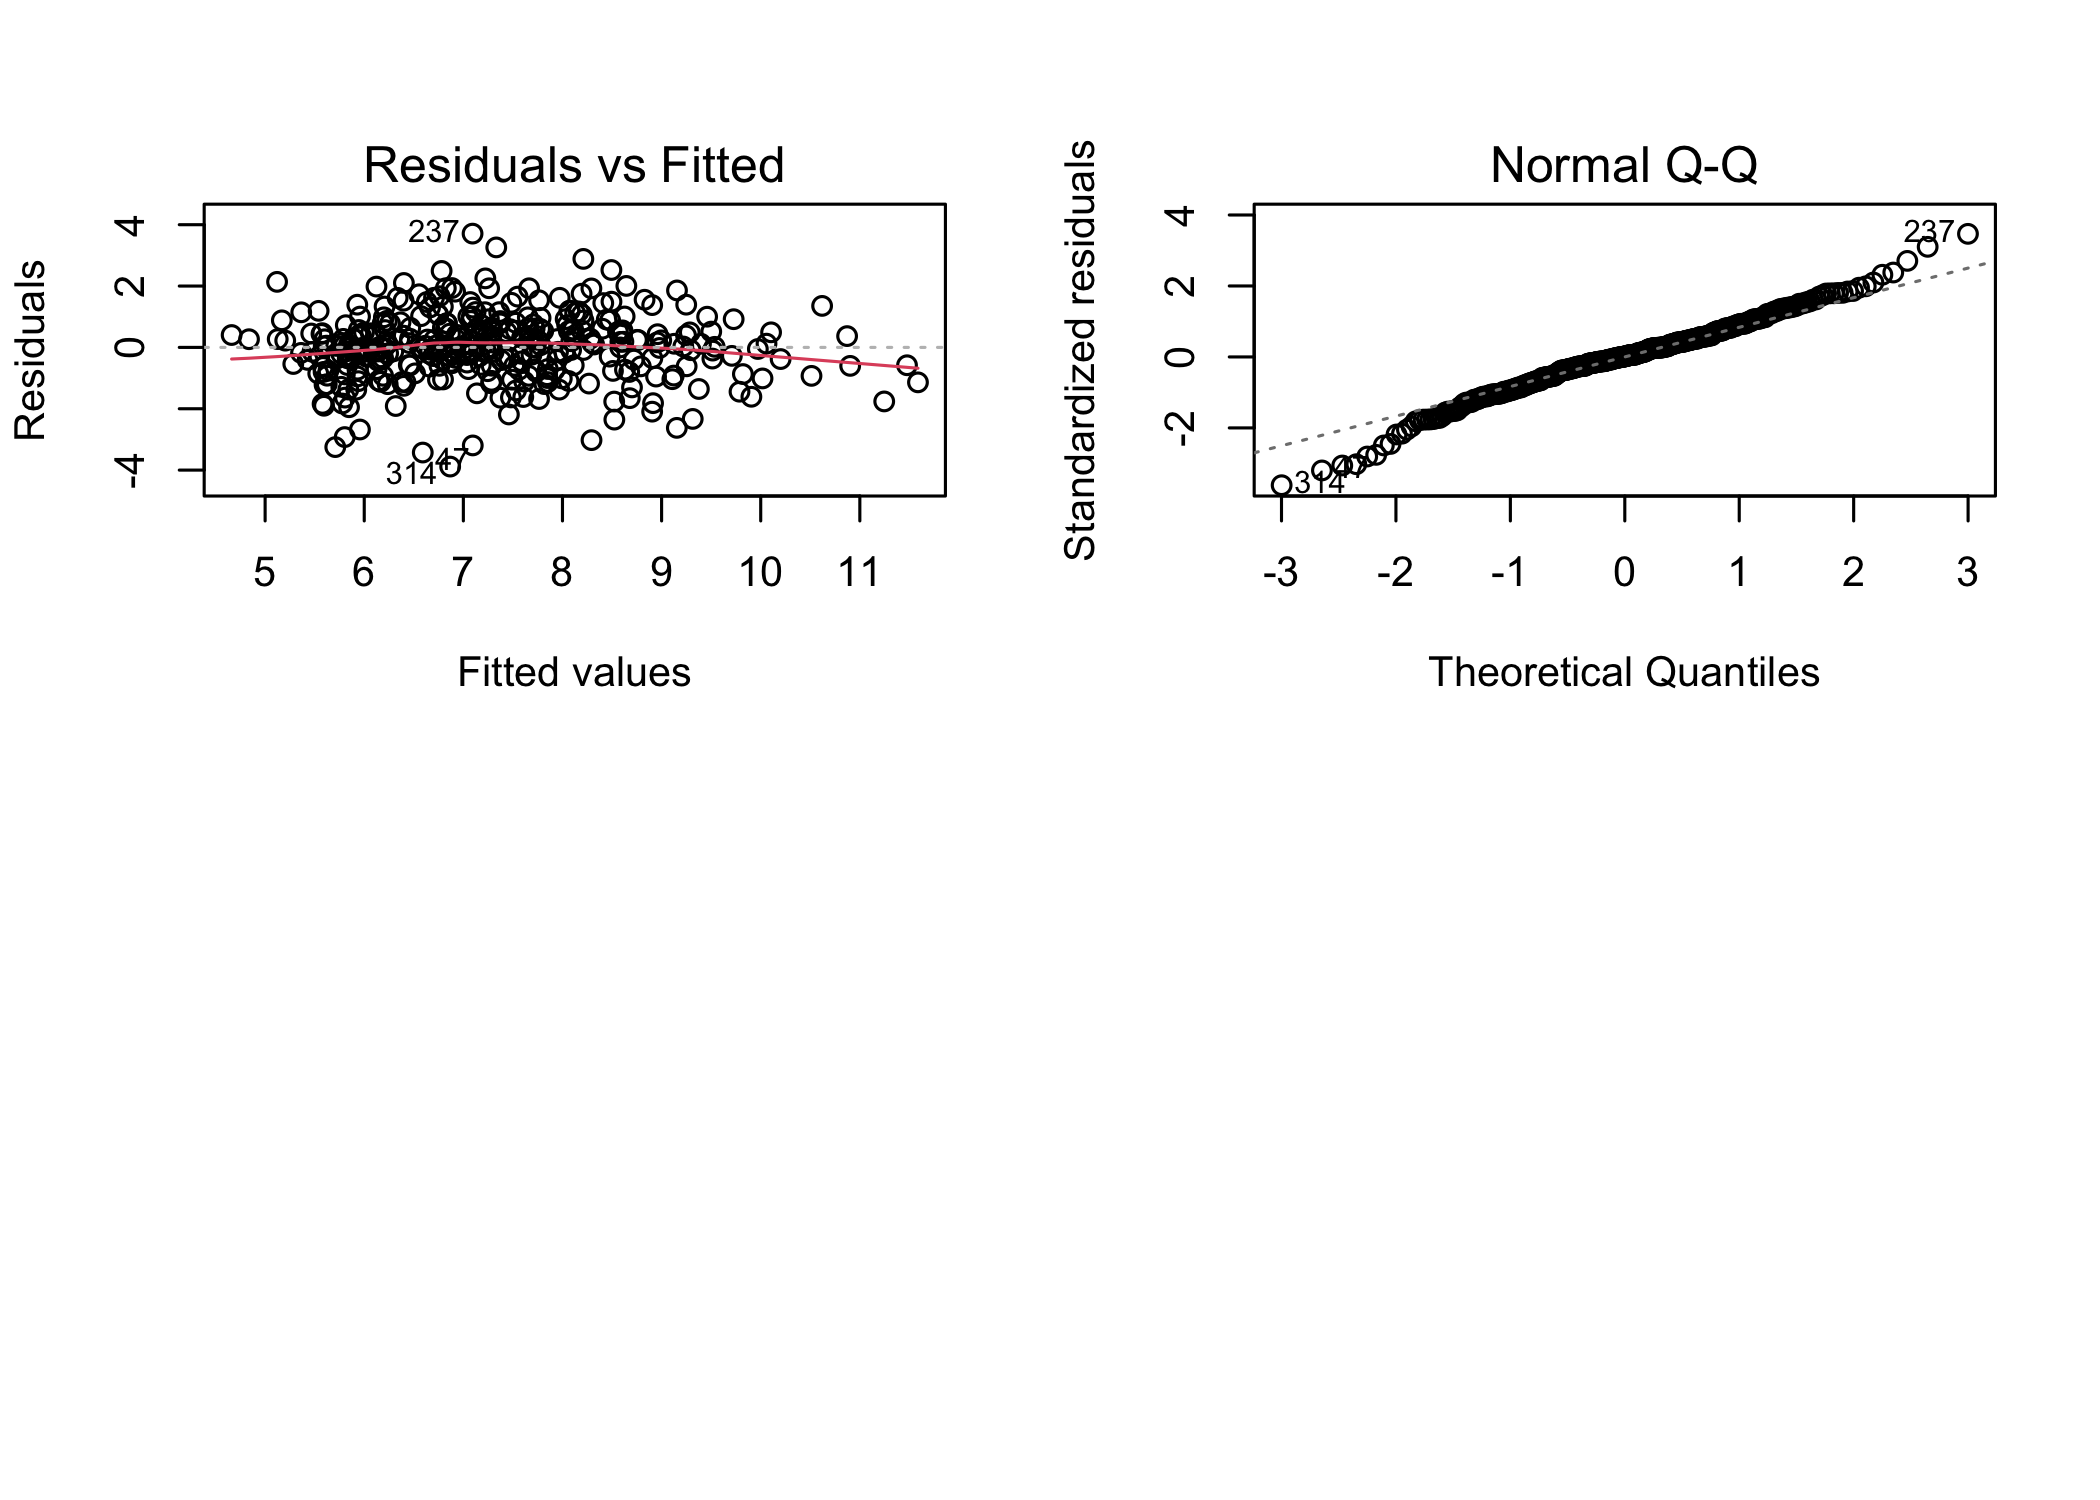
\includegraphics[width=0.9\linewidth]{main_files/figure-latex/unnamed-chunk-15-1} \caption{\label{fig:figs}Subset selection for best parameter numbers}\label{fig:unnamed-chunk-15}
\end{figure}

According to the output, we determine that the number of variables
should be above 12 because \(C_p \leq p\). Based on this analysis, we
find that \texttt{unemp} could also be selected.

\hypertarget{discussion}{%
\subsubsection{Discussion}\label{discussion}}

We need to remove totalinc, because it can be replaced. totalinc =
pcincome * pop.

\hypertarget{model-building-from-the-vairables-we-selected}{%
\subsection{Model building from the vairables we
selected}\label{model-building-from-the-vairables-we-selected}}

\begin{Shaded}
\begin{Highlighting}[]
\NormalTok{fit\_nest }\OtherTok{=} \FunctionTok{lm}\NormalTok{(crime\_rate\_1000 }\SpecialCharTok{\textasciitilde{}}  
\NormalTok{                  pop }\SpecialCharTok{+}\NormalTok{ pop18 }\SpecialCharTok{+}\NormalTok{ bagrad }\SpecialCharTok{+}
\NormalTok{                  poverty }\SpecialCharTok{+}\NormalTok{ unemp }\SpecialCharTok{+}\NormalTok{ pcincome }\SpecialCharTok{+}\NormalTok{ pcincome}\SpecialCharTok{*}\NormalTok{pop }\SpecialCharTok{+}\NormalTok{ region }\SpecialCharTok{+}
\NormalTok{                  beds\_rate\_1000 }\SpecialCharTok{+}\NormalTok{ density, }\AttributeTok{data =}\NormalTok{ cdi\_model)}
\FunctionTok{summary}\NormalTok{(fit\_nest)}
\end{Highlighting}
\end{Shaded}

\begin{verbatim}
## 
## Call:
## lm(formula = crime_rate_1000 ~ pop + pop18 + bagrad + poverty + 
##     unemp + pcincome + pcincome * pop + region + beds_rate_1000 + 
##     density, data = cdi_model)
## 
## Residuals:
##     Min      1Q  Median      3Q     Max 
## -43.123  -9.614  -1.011   8.440  57.956 
## 
## Coefficients:
##                  Estimate Std. Error t value Pr(>|t|)    
## (Intercept)    -8.318e+01  1.549e+01  -5.371 1.42e-07 ***
## pop             8.026e-05  1.335e-05   6.011 4.59e-09 ***
## pop18           1.250e+00  3.208e-01   3.894 0.000118 ***
## bagrad         -3.679e-01  2.519e-01  -1.461 0.145035    
## poverty         1.664e+00  3.909e-01   4.257 2.66e-05 ***
## unemp           7.482e-01  5.310e-01   1.409 0.159717    
## pcincome        3.198e-03  6.059e-04   5.277 2.29e-07 ***
## region2         1.203e+01  2.618e+00   4.597 5.98e-06 ***
## region3         2.967e+01  2.682e+00  11.065  < 2e-16 ***
## region4         2.463e+01  3.128e+00   7.873 4.27e-14 ***
## beds_rate_1000  3.088e+00  6.859e-01   4.502 9.14e-06 ***
## density         8.670e-04  6.738e-04   1.287 0.199066    
## pop:pcincome   -3.406e-09  6.500e-10  -5.240 2.76e-07 ***
## ---
## Signif. codes:  0 '***' 0.001 '**' 0.01 '*' 0.05 '.' 0.1 ' ' 1
## 
## Residual standard error: 16.22 on 354 degrees of freedom
## Multiple R-squared:  0.563,  Adjusted R-squared:  0.5482 
## F-statistic: 38.01 on 12 and 354 DF,  p-value: < 2.2e-16
\end{verbatim}

\begin{Shaded}
\begin{Highlighting}[]
\FunctionTok{par}\NormalTok{(}\AttributeTok{mfrow =} \FunctionTok{c}\NormalTok{(}\DecValTok{2}\NormalTok{,}\DecValTok{2}\NormalTok{))}
\FunctionTok{plot}\NormalTok{(fit\_nest)}
\end{Highlighting}
\end{Shaded}

\begin{figure}
\includegraphics[width=0.9\linewidth]{main_files/figure-latex/unnamed-chunk-17-1} \caption{\label{fig:figs}Diagnose plots of model without interaction terms}\label{fig:unnamed-chunk-17}
\end{figure}

\begin{Shaded}
\begin{Highlighting}[]
\FunctionTok{boxcox}\NormalTok{(fit\_nest)}
\end{Highlighting}
\end{Shaded}

\begin{figure}
\includegraphics[width=0.9\linewidth]{main_files/figure-latex/unnamed-chunk-18-1} \caption{\label{fig:figs}Boxcox plot of model without interaction terms}\label{fig:unnamed-chunk-18}
\end{figure}

The peak of boxcox plot is close to around 0.5\textasciitilde1. Try
\(\sqrt{y}\) transformation

\hypertarget{transformation}{%
\subsubsection{transformation}\label{transformation}}

\begin{Shaded}
\begin{Highlighting}[]
\NormalTok{cdi\_model\_trans }\OtherTok{=}\NormalTok{ cdi\_model }\SpecialCharTok{\%\textgreater{}\%} 
  \FunctionTok{mutate}\NormalTok{(}
    \AttributeTok{y\_sqrt =} \FunctionTok{sqrt}\NormalTok{(crime\_rate\_1000)}
\NormalTok{  )}

\NormalTok{fit\_nest\_trans }\OtherTok{=} \FunctionTok{lm}\NormalTok{(y\_sqrt }\SpecialCharTok{\textasciitilde{}}  
\NormalTok{                   pop }\SpecialCharTok{+}\NormalTok{ pop18 }\SpecialCharTok{+}\NormalTok{ bagrad }\SpecialCharTok{+}
\NormalTok{                  poverty }\SpecialCharTok{+}\NormalTok{ unemp }\SpecialCharTok{+}\NormalTok{ pcincome }\SpecialCharTok{+}\NormalTok{ pcincome}\SpecialCharTok{*}\NormalTok{pop }\SpecialCharTok{+}\NormalTok{ region }\SpecialCharTok{+}
\NormalTok{                  beds\_rate\_1000 }\SpecialCharTok{+}\NormalTok{ density, }\AttributeTok{data =}\NormalTok{ cdi\_model\_trans)}
\FunctionTok{summary}\NormalTok{(fit\_nest\_trans)}
\end{Highlighting}
\end{Shaded}

\begin{verbatim}
## 
## Call:
## lm(formula = y_sqrt ~ pop + pop18 + bagrad + poverty + unemp + 
##     pcincome + pcincome * pop + region + beds_rate_1000 + density, 
##     data = cdi_model_trans)
## 
## Residuals:
##     Min      1Q  Median      3Q     Max 
## -4.0165 -0.6220 -0.0030  0.6178  3.4444 
## 
## Coefficients:
##                  Estimate Std. Error t value Pr(>|t|)    
## (Intercept)    -1.813e+00  1.060e+00  -1.710 0.088124 .  
## pop             5.046e-06  9.142e-07   5.520 6.56e-08 ***
## pop18           8.223e-02  2.197e-02   3.744 0.000212 ***
## bagrad         -2.693e-02  1.725e-02  -1.562 0.119298    
## poverty         9.395e-02  2.677e-02   3.510 0.000506 ***
## unemp           5.976e-02  3.636e-02   1.644 0.101141    
## pcincome        2.049e-04  4.149e-05   4.938 1.22e-06 ***
## region2         8.599e-01  1.792e-01   4.798 2.37e-06 ***
## region3         2.098e+00  1.836e-01  11.427  < 2e-16 ***
## region4         1.863e+00  2.141e-01   8.700  < 2e-16 ***
## beds_rate_1000  2.227e-01  4.696e-02   4.742 3.07e-06 ***
## density         5.455e-05  4.613e-05   1.182 0.237840    
## pop:pcincome   -2.115e-10  4.450e-11  -4.753 2.93e-06 ***
## ---
## Signif. codes:  0 '***' 0.001 '**' 0.01 '*' 0.05 '.' 0.1 ' ' 1
## 
## Residual standard error: 1.11 on 354 degrees of freedom
## Multiple R-squared:  0.5515, Adjusted R-squared:  0.5363 
## F-statistic: 36.28 on 12 and 354 DF,  p-value: < 2.2e-16
\end{verbatim}

\begin{Shaded}
\begin{Highlighting}[]
\FunctionTok{par}\NormalTok{(}\AttributeTok{mfrow =} \FunctionTok{c}\NormalTok{(}\DecValTok{2}\NormalTok{,}\DecValTok{2}\NormalTok{))}
\FunctionTok{plot}\NormalTok{(fit\_nest\_trans)}
\end{Highlighting}
\end{Shaded}

\begin{figure}
\includegraphics[width=0.9\linewidth]{main_files/figure-latex/unnamed-chunk-20-1} \caption{\label{fig:figs}Diagnose plots of model without interaction terms}\label{fig:unnamed-chunk-20}
\end{figure}

Compare to the diagnose plots of untransformed model, we found that the
residuals are more unevenly distributed. Therefore, transformed model is
worse. We select the untransformed model.

Our first model: \[crime\_rate\_1000 = pop + pop18 + bagrad +
                  poverty + unemp \\ + pcincome + pcincome*pop + region
                  beds\_rate\_1000 + density\]

\hypertarget{add-interaction-term-povertyincome}{%
\subsection{Add Interaction term:
poverty+income}\label{add-interaction-term-povertyincome}}

According to Census Bureau, the number of persons below the official
government poverty level was 33.6 million in 1990, representing 13.5
percent of the Nation's population. Thus, we can use this criteria to
divide \texttt{poverty} into two category: higher than national poverty
rate and lower than national poverty rate.

\begin{Shaded}
\begin{Highlighting}[]
\NormalTok{poverty\_status }\OtherTok{=}\NormalTok{ cdi\_model }\SpecialCharTok{\%\textgreater{}\%} 
  \FunctionTok{mutate}\NormalTok{(}\AttributeTok{national\_poverty =} \FunctionTok{if\_else}\NormalTok{(poverty }\SpecialCharTok{\textgreater{}} \FloatTok{13.5}\NormalTok{, }\StringTok{"higher"}\NormalTok{, }\StringTok{"lower"}\NormalTok{))}

\FunctionTok{ggplot}\NormalTok{(poverty\_status, }\FunctionTok{aes}\NormalTok{(}\AttributeTok{x =}\NormalTok{ pcincome, }\AttributeTok{y =}\NormalTok{ crime\_rate\_1000, }\AttributeTok{color =}\NormalTok{ national\_poverty)) }\SpecialCharTok{+} 
  \FunctionTok{geom\_point}\NormalTok{(}\AttributeTok{alpha =}\NormalTok{ .}\DecValTok{5}\NormalTok{) }\SpecialCharTok{+}
  \FunctionTok{geom\_smooth}\NormalTok{(}\AttributeTok{method =} \StringTok{"lm"}\NormalTok{, }\AttributeTok{se =}\NormalTok{ F, }\FunctionTok{aes}\NormalTok{(}\AttributeTok{group =}\NormalTok{ national\_poverty, }\AttributeTok{color =}\NormalTok{ national\_poverty)) }\SpecialCharTok{+}
  \FunctionTok{labs}\NormalTok{(}
    \AttributeTok{title =} \StringTok{"Crime Rate and Per Capita Income by Poverty Status"}\NormalTok{,}
    \AttributeTok{x =} \StringTok{"Per Capita Income"}\NormalTok{,}
    \AttributeTok{y =} \StringTok{"Crime Rate "}\NormalTok{,}
    \AttributeTok{color =} \StringTok{"Comparison with national avergae"}
\NormalTok{  )}
\end{Highlighting}
\end{Shaded}

\begin{figure}
\includegraphics[width=0.9\linewidth]{main_files/figure-latex/unnamed-chunk-21-1} \caption{\label{fig:figs}Interaction plot of Income Per Capita and Poverty}\label{fig:unnamed-chunk-21}
\end{figure}

\begin{Shaded}
\begin{Highlighting}[]
\NormalTok{fit\_int1 }\OtherTok{=} \FunctionTok{lm}\NormalTok{(crime\_rate\_1000 }\SpecialCharTok{\textasciitilde{}}  
\NormalTok{                   pop }\SpecialCharTok{+}\NormalTok{ pop18 }\SpecialCharTok{+}\NormalTok{ bagrad }\SpecialCharTok{+}
\NormalTok{                  poverty }\SpecialCharTok{+}\NormalTok{ unemp }\SpecialCharTok{+}\NormalTok{ pcincome }\SpecialCharTok{+}\NormalTok{ pcincome}\SpecialCharTok{*}\NormalTok{pop }\SpecialCharTok{+}\NormalTok{ region }\SpecialCharTok{+}
\NormalTok{                  beds\_rate\_1000 }\SpecialCharTok{+}\NormalTok{ density }\SpecialCharTok{+}
\NormalTok{                  poverty}\SpecialCharTok{*}\NormalTok{pcincome, }\AttributeTok{data =}\NormalTok{ cdi\_model)}
\FunctionTok{summary}\NormalTok{(fit\_int1) }\SpecialCharTok{\%\textgreater{}\%}\NormalTok{ broom}\SpecialCharTok{::}\FunctionTok{tidy}\NormalTok{()}
\end{Highlighting}
\end{Shaded}

\begin{verbatim}
## # A tibble: 14 x 5
##    term             estimate std.error statistic  p.value
##    <chr>               <dbl>     <dbl>     <dbl>    <dbl>
##  1 (Intercept)      -4.88e+1  1.75e+ 1    -2.80  5.46e- 3
##  2 pop               6.17e-5  1.39e- 5     4.44  1.19e- 5
##  3 pop18             1.14e+0  3.16e- 1     3.60  3.57e- 4
##  4 bagrad           -2.62e-1  2.48e- 1    -1.05  2.93e- 1
##  5 poverty          -2.54e+0  1.12e+ 0    -2.26  2.46e- 2
##  6 unemp             7.42e-1  5.20e- 1     1.43  1.55e- 1
##  7 pcincome          1.42e-3  7.43e- 4     1.91  5.72e- 2
##  8 region2           1.07e+1  2.59e+ 0     4.15  4.20e- 5
##  9 region3           2.80e+1  2.66e+ 0    10.5   1.19e-22
## 10 region4           2.22e+1  3.13e+ 0     7.08  7.60e-12
## 11 beds_rate_1000    2.01e+0  7.25e- 1     2.77  5.91e- 3
## 12 density           2.01e-4  6.81e- 4     0.295 7.68e- 1
## 13 pop:pcincome     -2.56e-9  6.71e-10    -3.82  1.59e- 4
## 14 poverty:pcincome  2.80e-4  7.05e- 5     3.98  8.52e- 5
\end{verbatim}

\begin{Shaded}
\begin{Highlighting}[]
\FunctionTok{check\_collinearity}\NormalTok{(fit\_int1)}
\end{Highlighting}
\end{Shaded}

\begin{verbatim}
## # Check for Multicollinearity
## 
## Low Correlation
## 
##              Term  VIF Increased SE Tolerance
##               pop 1.00         1.00      1.00
##             pop18 2.10         1.45      0.48
##            bagrad 2.61         1.62      0.38
##           poverty 1.18         1.09      0.85
##             unemp 1.69         1.30      0.59
##          pcincome 1.12         1.06      0.89
##            region 1.59         1.26      0.63
##    beds_rate_1000 1.38         1.18      0.72
##           density 1.01         1.01      0.99
##      pop:pcincome 1.00         1.00      1.00
##  poverty:pcincome 1.00         1.00      1.00
\end{verbatim}

We notice that \texttt{density}, \texttt{bagrad} are not significant

\begin{Shaded}
\begin{Highlighting}[]
\CommentTok{\# remove density}
\NormalTok{fit\_int1 }\OtherTok{=} \FunctionTok{lm}\NormalTok{(crime\_rate\_1000 }\SpecialCharTok{\textasciitilde{}}  
\NormalTok{                   pop }\SpecialCharTok{+}\NormalTok{ pop18 }\SpecialCharTok{+}\NormalTok{ bagrad }\SpecialCharTok{+}
\NormalTok{                  poverty }\SpecialCharTok{+}\NormalTok{ unemp }\SpecialCharTok{+}\NormalTok{ pcincome }\SpecialCharTok{+}\NormalTok{ pcincome}\SpecialCharTok{*}\NormalTok{pop }\SpecialCharTok{+}\NormalTok{ region }\SpecialCharTok{+}
\NormalTok{                  beds\_rate\_1000  }\SpecialCharTok{+}
\NormalTok{                  poverty}\SpecialCharTok{*}\NormalTok{pcincome, }\AttributeTok{data =}\NormalTok{ cdi\_model)}
\FunctionTok{summary}\NormalTok{(fit\_int1)}
\end{Highlighting}
\end{Shaded}

\begin{verbatim}
## 
## Call:
## lm(formula = crime_rate_1000 ~ pop + pop18 + bagrad + poverty + 
##     unemp + pcincome + pcincome * pop + region + beds_rate_1000 + 
##     poverty * pcincome, data = cdi_model)
## 
## Residuals:
##     Min      1Q  Median      3Q     Max 
## -44.560  -8.893  -0.811   8.674  64.139 
## 
## Coefficients:
##                    Estimate Std. Error t value Pr(>|t|)    
## (Intercept)      -4.943e+01  1.731e+01  -2.855 0.004553 ** 
## pop               6.171e-05  1.387e-05   4.448 1.16e-05 ***
## pop18             1.153e+00  3.109e-01   3.708 0.000242 ***
## bagrad           -2.687e-01  2.467e-01  -1.089 0.276790    
## poverty          -2.594e+00  1.107e+00  -2.342 0.019719 *  
## unemp             7.393e-01  5.195e-01   1.423 0.155595    
## pcincome          1.431e-03  7.414e-04   1.930 0.054403 .  
## region2           1.067e+01  2.575e+00   4.143 4.29e-05 ***
## region3           2.790e+01  2.647e+00  10.539  < 2e-16 ***
## region4           2.207e+01  3.110e+00   7.096 7.03e-12 ***
## beds_rate_1000    2.004e+00  7.238e-01   2.768 0.005932 ** 
## pop:pcincome     -2.555e-09  6.699e-10  -3.814 0.000161 ***
## poverty:pcincome  2.856e-04  6.829e-05   4.182 3.65e-05 ***
## ---
## Signif. codes:  0 '***' 0.001 '**' 0.01 '*' 0.05 '.' 0.1 ' ' 1
## 
## Residual standard error: 15.87 on 354 degrees of freedom
## Multiple R-squared:  0.5816, Adjusted R-squared:  0.5674 
## F-statistic: 41.01 on 12 and 354 DF,  p-value: < 2.2e-16
\end{verbatim}

\begin{Shaded}
\begin{Highlighting}[]
\FunctionTok{check\_collinearity}\NormalTok{(fit\_int1)}
\end{Highlighting}
\end{Shaded}

\begin{verbatim}
## # Check for Multicollinearity
## 
## Low Correlation
## 
##              Term  VIF Increased SE Tolerance
##               pop 1.00         1.00      1.00
##             pop18 2.08         1.44      0.48
##            bagrad 2.59         1.61      0.39
##           poverty 1.18         1.09      0.85
##             unemp 1.69         1.30      0.59
##          pcincome 1.13         1.06      0.89
##            region 1.59         1.26      0.63
##    beds_rate_1000 1.39         1.18      0.72
##      pop:pcincome 1.00         1.00      1.00
##  poverty:pcincome 1.00         1.00      1.00
\end{verbatim}

\begin{Shaded}
\begin{Highlighting}[]
\CommentTok{\# remove bagrad}
\NormalTok{fit\_int1 }\OtherTok{=} \FunctionTok{lm}\NormalTok{(crime\_rate\_1000 }\SpecialCharTok{\textasciitilde{}}  
\NormalTok{                   pop }\SpecialCharTok{+}\NormalTok{ pop18 }\SpecialCharTok{+} 
\NormalTok{                  poverty }\SpecialCharTok{+}\NormalTok{ unemp }\SpecialCharTok{+}\NormalTok{ pcincome }\SpecialCharTok{+}\NormalTok{ pcincome}\SpecialCharTok{*}\NormalTok{pop }\SpecialCharTok{+}\NormalTok{ region }\SpecialCharTok{+}
\NormalTok{                  beds\_rate\_1000  }\SpecialCharTok{+}
\NormalTok{                  poverty}\SpecialCharTok{*}\NormalTok{pcincome, }\AttributeTok{data =}\NormalTok{ cdi\_model)}
\FunctionTok{summary}\NormalTok{(fit\_int1)}
\end{Highlighting}
\end{Shaded}

\begin{verbatim}
## 
## Call:
## lm(formula = crime_rate_1000 ~ pop + pop18 + poverty + unemp + 
##     pcincome + pcincome * pop + region + beds_rate_1000 + poverty * 
##     pcincome, data = cdi_model)
## 
## Residuals:
##     Min      1Q  Median      3Q     Max 
## -45.933  -8.984  -0.825   9.062  64.974 
## 
## Coefficients:
##                    Estimate Std. Error t value Pr(>|t|)    
## (Intercept)      -4.143e+01  1.568e+01  -2.642 0.008603 ** 
## pop               6.001e-05  1.379e-05   4.352 1.76e-05 ***
## pop18             9.277e-01  2.321e-01   3.996 7.84e-05 ***
## poverty          -2.777e+00  1.095e+00  -2.536 0.011647 *  
## unemp             9.432e-01  4.847e-01   1.946 0.052468 .  
## pcincome          9.798e-04  6.151e-04   1.593 0.112068    
## region2           1.079e+01  2.573e+00   4.194 3.47e-05 ***
## region3           2.769e+01  2.641e+00  10.485  < 2e-16 ***
## region4           2.132e+01  3.033e+00   7.028 1.08e-11 ***
## beds_rate_1000    1.988e+00  7.238e-01   2.746 0.006339 ** 
## pop:pcincome     -2.457e-09  6.640e-10  -3.700 0.000249 ***
## poverty:pcincome  2.957e-04  6.766e-05   4.371 1.63e-05 ***
## ---
## Signif. codes:  0 '***' 0.001 '**' 0.01 '*' 0.05 '.' 0.1 ' ' 1
## 
## Residual standard error: 15.87 on 355 degrees of freedom
## Multiple R-squared:  0.5802, Adjusted R-squared:  0.5672 
## F-statistic: 44.61 on 11 and 355 DF,  p-value: < 2.2e-16
\end{verbatim}

\begin{Shaded}
\begin{Highlighting}[]
\FunctionTok{check\_collinearity}\NormalTok{(fit\_int1)}
\end{Highlighting}
\end{Shaded}

\begin{verbatim}
## # Check for Multicollinearity
## 
## Low Correlation
## 
##              Term  VIF Increased SE Tolerance
##               pop 1.00         1.00      1.00
##             pop18 1.16         1.08      0.86
##           poverty 1.17         1.08      0.86
##             unemp 1.47         1.21      0.68
##          pcincome 1.09         1.04      0.92
##            region 1.47         1.21      0.68
##    beds_rate_1000 1.39         1.18      0.72
##      pop:pcincome 1.00         1.00      1.00
##  poverty:pcincome 1.00         1.00      1.00
\end{verbatim}

\hypertarget{diagnose}{%
\subsubsection{diagnose}\label{diagnose}}

\begin{Shaded}
\begin{Highlighting}[]
\FunctionTok{par}\NormalTok{(}\AttributeTok{mfrow =} \FunctionTok{c}\NormalTok{(}\DecValTok{2}\NormalTok{,}\DecValTok{2}\NormalTok{))}
\FunctionTok{plot}\NormalTok{(fit\_int1)}
\end{Highlighting}
\end{Shaded}

\begin{figure}
\includegraphics[width=0.9\linewidth]{main_files/figure-latex/unnamed-chunk-25-1} \caption{\label{fig:figs}Diagnose plots with interaction terms:poverty*pcincome}\label{fig:unnamed-chunk-25}
\end{figure}

\begin{Shaded}
\begin{Highlighting}[]
\FunctionTok{boxcox}\NormalTok{(fit\_int1)}
\end{Highlighting}
\end{Shaded}

\begin{figure}
\includegraphics[width=0.9\linewidth]{main_files/figure-latex/unnamed-chunk-26-1} \caption{\label{fig:figs}Boxcox plot with interaction terms:poverty*pcincome}\label{fig:unnamed-chunk-26}
\end{figure}

The peak of boxcox plot is close to around 0.5\textasciitilde1. Try
\(\sqrt{y}\) transformation

\hypertarget{transformation-1}{%
\subsubsection{transformation}\label{transformation-1}}

\begin{Shaded}
\begin{Highlighting}[]
\NormalTok{cdi\_model\_trans }\OtherTok{=}\NormalTok{ cdi\_model }\SpecialCharTok{\%\textgreater{}\%} 
  \FunctionTok{mutate}\NormalTok{(}
    \AttributeTok{y\_sqrt =} \FunctionTok{sqrt}\NormalTok{(crime\_rate\_1000)}
\NormalTok{  )}

\NormalTok{fit\_int1\_trans }\OtherTok{=} \FunctionTok{lm}\NormalTok{(y\_sqrt }\SpecialCharTok{\textasciitilde{}}  
\NormalTok{                   pop }\SpecialCharTok{+}\NormalTok{ pop18 }\SpecialCharTok{+} 
\NormalTok{                  poverty }\SpecialCharTok{+}\NormalTok{ unemp }\SpecialCharTok{+}\NormalTok{ pcincome }\SpecialCharTok{+}\NormalTok{ pcincome}\SpecialCharTok{*}\NormalTok{pop }\SpecialCharTok{+}\NormalTok{ region }\SpecialCharTok{+}
\NormalTok{                  beds\_rate\_1000  }\SpecialCharTok{+}
\NormalTok{                  poverty}\SpecialCharTok{*}\NormalTok{pcincome, }\AttributeTok{data =}\NormalTok{ cdi\_model\_trans)}
\FunctionTok{summary}\NormalTok{(fit\_int1\_trans)}
\end{Highlighting}
\end{Shaded}

\begin{verbatim}
## 
## Call:
## lm(formula = y_sqrt ~ pop + pop18 + poverty + unemp + pcincome + 
##     pcincome * pop + region + beds_rate_1000 + poverty * pcincome, 
##     data = cdi_model_trans)
## 
## Residuals:
##     Min      1Q  Median      3Q     Max 
## -3.9383 -0.5569  0.0166  0.6563  3.7968 
## 
## Coefficients:
##                    Estimate Std. Error t value Pr(>|t|)    
## (Intercept)       9.271e-01  1.078e+00   0.860 0.390234    
## pop               3.748e-06  9.476e-07   3.955 9.24e-05 ***
## pop18             5.881e-02  1.596e-02   3.686 0.000264 ***
## poverty          -1.882e-01  7.525e-02  -2.500 0.012857 *  
## unemp             7.489e-02  3.331e-02   2.248 0.025191 *  
## pcincome          5.891e-05  4.228e-05   1.394 0.164333    
## region2           7.833e-01  1.768e-01   4.430 1.26e-05 ***
## region3           1.970e+00  1.815e-01  10.855  < 2e-16 ***
## region4           1.644e+00  2.085e-01   7.888 3.84e-14 ***
## beds_rate_1000    1.532e-01  4.975e-02   3.079 0.002236 ** 
## pop:pcincome     -1.504e-10  4.563e-11  -3.295 0.001084 ** 
## poverty:pcincome  1.876e-05  4.650e-06   4.034 6.71e-05 ***
## ---
## Signif. codes:  0 '***' 0.001 '**' 0.01 '*' 0.05 '.' 0.1 ' ' 1
## 
## Residual standard error: 1.091 on 355 degrees of freedom
## Multiple R-squared:  0.5659, Adjusted R-squared:  0.5524 
## F-statistic: 42.07 on 11 and 355 DF,  p-value: < 2.2e-16
\end{verbatim}

\begin{Shaded}
\begin{Highlighting}[]
\FunctionTok{par}\NormalTok{(}\AttributeTok{mfrow =} \FunctionTok{c}\NormalTok{(}\DecValTok{2}\NormalTok{,}\DecValTok{2}\NormalTok{))}
\FunctionTok{plot}\NormalTok{(fit\_int1\_trans)}
\end{Highlighting}
\end{Shaded}

\begin{figure}
\includegraphics[width=0.9\linewidth]{main_files/figure-latex/unnamed-chunk-28-1} \caption{\label{fig:figs}Diagnose plots with interaction terms:poverty*pcincome}\label{fig:unnamed-chunk-28}
\end{figure}

Compare to the diagnose plots of untransformed model, we found that the
residuals are more unevenly distributed. Therefore, transformed model is
worse. We select the untransformed model.

Our second model: \[crime\_rate\_1000 = pop + pop18 + 
                  poverty + unemp + pcincome + \\ pcincome*pop + region +
                  beds\_rate\_1000  +
                  poverty*pcincome\]

\hypertarget{add-interaction-term-pcincome-bagrad}{%
\subsection{Add interaction term: pcincome +
bagrad}\label{add-interaction-term-pcincome-bagrad}}

According to Census Bureau, national percent of persons 25 years old or
older with bachelor's degrees is 20.8\%. Thus, we can use this criteria
to divide \texttt{bagrad} into two category: higher than national
\texttt{bagrad} and lower than national \texttt{bargrad}.

\begin{Shaded}
\begin{Highlighting}[]
\NormalTok{bagrad\_status }\OtherTok{=}\NormalTok{ cdi\_model }\SpecialCharTok{\%\textgreater{}\%} 
  \FunctionTok{mutate}\NormalTok{(}\AttributeTok{national\_bagrad =} \FunctionTok{if\_else}\NormalTok{(bagrad }\SpecialCharTok{\textgreater{}} \FloatTok{20.8}\NormalTok{, }\StringTok{"higher"}\NormalTok{, }\StringTok{"lower"}\NormalTok{))}

\FunctionTok{ggplot}\NormalTok{(bagrad\_status, }\FunctionTok{aes}\NormalTok{(}\AttributeTok{x =}\NormalTok{ pcincome, }\AttributeTok{y =}\NormalTok{ crime\_rate\_1000, }\AttributeTok{color =}\NormalTok{ national\_bagrad)) }\SpecialCharTok{+} 
  \FunctionTok{geom\_point}\NormalTok{(}\AttributeTok{alpha =}\NormalTok{ .}\DecValTok{5}\NormalTok{) }\SpecialCharTok{+}
  \FunctionTok{geom\_smooth}\NormalTok{(}\AttributeTok{method =} \StringTok{"lm"}\NormalTok{, }\AttributeTok{se =}\NormalTok{ F, }\FunctionTok{aes}\NormalTok{(}\AttributeTok{group =}\NormalTok{ national\_bagrad, }\AttributeTok{color =}\NormalTok{ national\_bagrad)) }\SpecialCharTok{+}
  \FunctionTok{ylim}\NormalTok{(}\DecValTok{0}\NormalTok{,}\DecValTok{150}\NormalTok{) }\SpecialCharTok{+}
  \FunctionTok{labs}\NormalTok{(}
    \AttributeTok{title =} \StringTok{"Crime Rate and Per Capita Income by Percent Bachelor\textquotesingle{}s Degrees Status"}\NormalTok{,}
    \AttributeTok{x =} \StringTok{"Per Capita Income"}\NormalTok{,}
    \AttributeTok{y =} \StringTok{"Crime Rate"}\NormalTok{,}
    \AttributeTok{color =} \StringTok{"Comparison with national avergae"}
\NormalTok{  )}
\end{Highlighting}
\end{Shaded}

\begin{figure}
\includegraphics[width=0.9\linewidth]{main_files/figure-latex/unnamed-chunk-29-1} \caption{\label{fig:figs}Interaction plot of Income Per Capita and Bachelor's Degree Status}\label{fig:unnamed-chunk-29}
\end{figure}

\begin{Shaded}
\begin{Highlighting}[]
\NormalTok{fit\_int2 }\OtherTok{=} \FunctionTok{lm}\NormalTok{(crime\_rate\_1000 }\SpecialCharTok{\textasciitilde{}}  
\NormalTok{                  pop }\SpecialCharTok{+}\NormalTok{ pop18 }\SpecialCharTok{+}\NormalTok{ bagrad }\SpecialCharTok{+}
\NormalTok{                  poverty }\SpecialCharTok{+}\NormalTok{ unemp }\SpecialCharTok{+}\NormalTok{ pcincome }\SpecialCharTok{+}\NormalTok{ pcincome}\SpecialCharTok{*}\NormalTok{pop }\SpecialCharTok{+}\NormalTok{ region }\SpecialCharTok{+}
\NormalTok{                  beds\_rate\_1000 }\SpecialCharTok{+}\NormalTok{ density }\SpecialCharTok{+}
\NormalTok{                  pcincome}\SpecialCharTok{*}\NormalTok{bagrad, }\AttributeTok{data =}\NormalTok{ cdi\_model)}
\FunctionTok{summary}\NormalTok{(fit\_int2)}
\end{Highlighting}
\end{Shaded}

\begin{verbatim}
## 
## Call:
## lm(formula = crime_rate_1000 ~ pop + pop18 + bagrad + poverty + 
##     unemp + pcincome + pcincome * pop + region + beds_rate_1000 + 
##     density + pcincome * bagrad, data = cdi_model)
## 
## Residuals:
##    Min     1Q Median     3Q    Max 
## -42.88  -9.84  -0.85   8.19  61.74 
## 
## Coefficients:
##                   Estimate Std. Error t value Pr(>|t|)    
## (Intercept)     -1.141e+02  1.963e+01  -5.814 1.37e-08 ***
## pop              6.518e-05  1.453e-05   4.487 9.79e-06 ***
## pop18            1.048e+00  3.282e-01   3.193 0.001537 ** 
## bagrad           1.252e+00  6.865e-01   1.824 0.069046 .  
## poverty          1.906e+00  3.995e-01   4.770 2.69e-06 ***
## unemp            9.002e-01  5.304e-01   1.697 0.090555 .  
## pcincome         5.012e-03  9.351e-04   5.360 1.51e-07 ***
## region2          1.244e+01  2.603e+00   4.778 2.60e-06 ***
## region3          2.979e+01  2.662e+00  11.191  < 2e-16 ***
## region4          2.432e+01  3.107e+00   7.827 5.87e-14 ***
## beds_rate_1000   2.740e+00  6.944e-01   3.946 9.58e-05 ***
## density          1.007e-03  6.710e-04   1.500 0.134491    
## pop:pcincome    -2.706e-09  7.018e-10  -3.856 0.000137 ***
## bagrad:pcincome -8.009e-05  3.161e-05  -2.534 0.011723 *  
## ---
## Signif. codes:  0 '***' 0.001 '**' 0.01 '*' 0.05 '.' 0.1 ' ' 1
## 
## Residual standard error: 16.09 on 353 degrees of freedom
## Multiple R-squared:  0.5708, Adjusted R-squared:  0.555 
## F-statistic: 36.11 on 13 and 353 DF,  p-value: < 2.2e-16
\end{verbatim}

\begin{Shaded}
\begin{Highlighting}[]
\FunctionTok{check\_collinearity}\NormalTok{(fit\_int2)}
\end{Highlighting}
\end{Shaded}

\begin{verbatim}
## # Check for Multicollinearity
## 
## Low Correlation
## 
##             Term  VIF Increased SE Tolerance
##              pop 1.00         1.00      1.00
##            pop18 1.38         1.17      0.72
##           bagrad 1.63         1.27      0.62
##          poverty 1.96         1.40      0.51
##            unemp 1.46         1.21      0.69
##         pcincome 1.14         1.07      0.87
##           region 1.51         1.23      0.66
##   beds_rate_1000 1.82         1.35      0.55
##          density 1.02         1.01      0.98
##     pop:pcincome 1.00         1.00      1.00
##  bagrad:pcincome 1.00         1.00      1.00
\end{verbatim}

\hypertarget{diagnose-1}{%
\subsubsection{diagnose}\label{diagnose-1}}

\begin{Shaded}
\begin{Highlighting}[]
\FunctionTok{par}\NormalTok{(}\AttributeTok{mfrow =} \FunctionTok{c}\NormalTok{(}\DecValTok{2}\NormalTok{,}\DecValTok{2}\NormalTok{))}
\FunctionTok{plot}\NormalTok{(fit\_int2)}
\end{Highlighting}
\end{Shaded}

\begin{figure}
\includegraphics[width=0.9\linewidth]{main_files/figure-latex/unnamed-chunk-31-1} \caption{\label{fig:figs}Diagnose plots with interaction terms:pcincome*bagrad}\label{fig:unnamed-chunk-31}
\end{figure}

\begin{Shaded}
\begin{Highlighting}[]
\FunctionTok{boxcox}\NormalTok{(fit\_int2)}
\end{Highlighting}
\end{Shaded}

\begin{figure}
\includegraphics[width=0.9\linewidth]{main_files/figure-latex/unnamed-chunk-32-1} \caption{\label{fig:figs}Boxcox plot with interaction terms:pcincome*bagrad}\label{fig:unnamed-chunk-32}
\end{figure}

The peak of boxcox plot is close to around 0.5\textasciitilde1. Try
\(\sqrt{y}\) transformation

\hypertarget{transformation-2}{%
\subsubsection{transformation}\label{transformation-2}}

\begin{Shaded}
\begin{Highlighting}[]
\NormalTok{fit\_int2\_trans }\OtherTok{=} \FunctionTok{lm}\NormalTok{(y\_sqrt }\SpecialCharTok{\textasciitilde{}}  
\NormalTok{                  pop }\SpecialCharTok{+}\NormalTok{ pop18 }\SpecialCharTok{+}\NormalTok{ bagrad }\SpecialCharTok{+}
\NormalTok{                  poverty }\SpecialCharTok{+}\NormalTok{ unemp }\SpecialCharTok{+}\NormalTok{ pcincome }\SpecialCharTok{+}\NormalTok{ pcincome}\SpecialCharTok{*}\NormalTok{pop }\SpecialCharTok{+}\NormalTok{ region }\SpecialCharTok{+}
\NormalTok{                  beds\_rate\_1000 }\SpecialCharTok{+}\NormalTok{ density }\SpecialCharTok{+}
\NormalTok{                  pcincome}\SpecialCharTok{*}\NormalTok{bagrad, }\AttributeTok{data =}\NormalTok{ cdi\_model\_trans)}
\FunctionTok{summary}\NormalTok{(fit\_int2\_trans)}
\end{Highlighting}
\end{Shaded}

\begin{verbatim}
## 
## Call:
## lm(formula = y_sqrt ~ pop + pop18 + bagrad + poverty + unemp + 
##     pcincome + pcincome * pop + region + beds_rate_1000 + density + 
##     pcincome * bagrad, data = cdi_model_trans)
## 
## Residuals:
##     Min      1Q  Median      3Q     Max 
## -3.9297 -0.6537 -0.0077  0.6205  3.6242 
## 
## Coefficients:
##                   Estimate Std. Error t value Pr(>|t|)    
## (Intercept)     -4.111e+00  1.342e+00  -3.064 0.002351 ** 
## pop              3.926e-06  9.930e-07   3.954 9.28e-05 ***
## pop18            6.725e-02  2.244e-02   2.998 0.002914 ** 
## bagrad           9.341e-02  4.693e-02   1.990 0.047307 *  
## poverty          1.119e-01  2.731e-02   4.098 5.18e-05 ***
## unemp            7.105e-02  3.626e-02   1.960 0.050833 .  
## pcincome         3.396e-04  6.392e-05   5.314 1.91e-07 ***
## region2          8.899e-01  1.779e-01   5.002 8.98e-07 ***
## region3          2.107e+00  1.820e-01  11.577  < 2e-16 ***
## region4          1.840e+00  2.123e-01   8.666  < 2e-16 ***
## beds_rate_1000   1.968e-01  4.746e-02   4.147 4.22e-05 ***
## density          6.492e-05  4.587e-05   1.415 0.157840    
## pop:pcincome    -1.595e-10  4.797e-11  -3.325 0.000978 ***
## bagrad:pcincome -5.950e-06  2.161e-06  -2.753 0.006202 ** 
## ---
## Signif. codes:  0 '***' 0.001 '**' 0.01 '*' 0.05 '.' 0.1 ' ' 1
## 
## Residual standard error: 1.1 on 353 degrees of freedom
## Multiple R-squared:  0.561,  Adjusted R-squared:  0.5448 
## F-statistic: 34.69 on 13 and 353 DF,  p-value: < 2.2e-16
\end{verbatim}

\begin{Shaded}
\begin{Highlighting}[]
\FunctionTok{par}\NormalTok{(}\AttributeTok{mfrow =} \FunctionTok{c}\NormalTok{(}\DecValTok{2}\NormalTok{,}\DecValTok{2}\NormalTok{))}
\FunctionTok{plot}\NormalTok{(fit\_int2\_trans)}
\end{Highlighting}
\end{Shaded}

\begin{figure}
\includegraphics[width=0.9\linewidth]{main_files/figure-latex/unnamed-chunk-34-1} \caption{\label{fig:figs}Diagnose plots with interaction terms:pcincome*bagrad}\label{fig:unnamed-chunk-34}
\end{figure}

Compare to the diagnose plots of untransformed model, we found that the
residuals are more unevenly distributed. Therefore, transformed model is
worse. We select the untransformed model.

Our third model: \[crime\_rate\_1000 = pop + pop18 + bagrad +
                  poverty + unemp + pcincome + \\ pcincome*pop + region +
                  beds\_rate\_1000 + density +
                  pcincome*bagrad\]\\
\#\# Cross validation

\hypertarget{model-1}{%
\subsubsection{model 1}\label{model-1}}

\begin{Shaded}
\begin{Highlighting}[]
\FunctionTok{set.seed}\NormalTok{(}\DecValTok{1}\NormalTok{)}
\NormalTok{train }\OtherTok{=} \FunctionTok{trainControl}\NormalTok{(}\AttributeTok{method =} \StringTok{"cv"}\NormalTok{, }\AttributeTok{number =} \DecValTok{5}\NormalTok{)}

\NormalTok{model\_train1 }\OtherTok{=} \FunctionTok{train}\NormalTok{(crime\_rate\_1000 }\SpecialCharTok{\textasciitilde{}}  
\NormalTok{                  pop }\SpecialCharTok{+}\NormalTok{ pop18 }\SpecialCharTok{+}\NormalTok{ bagrad }\SpecialCharTok{+}
\NormalTok{                  poverty }\SpecialCharTok{+}\NormalTok{ unemp }\SpecialCharTok{+}\NormalTok{ pcincome }\SpecialCharTok{+}\NormalTok{ pcincome}\SpecialCharTok{*}\NormalTok{pop }\SpecialCharTok{+}\NormalTok{ region }\SpecialCharTok{+}
\NormalTok{                  beds\_rate\_1000 }\SpecialCharTok{+}\NormalTok{ density,}\AttributeTok{data =}\NormalTok{ cdi\_model,}
                   \AttributeTok{trControl =}\NormalTok{ train,}
                   \AttributeTok{method =} \StringTok{\textquotesingle{}lm\textquotesingle{}}\NormalTok{,}
                   \AttributeTok{na.action =}\NormalTok{ na.pass)}
\FunctionTok{print}\NormalTok{(model\_train1)}
\end{Highlighting}
\end{Shaded}

\begin{verbatim}
## Linear Regression 
## 
## 367 samples
##   9 predictor
## 
## No pre-processing
## Resampling: Cross-Validated (5 fold) 
## Summary of sample sizes: 293, 294, 294, 294, 293 
## Resampling results:
## 
##   RMSE      Rsquared   MAE     
##   16.60425  0.5343078  12.52969
## 
## Tuning parameter 'intercept' was held constant at a value of TRUE
\end{verbatim}

\hypertarget{model-2}{%
\subsubsection{model 2}\label{model-2}}

\begin{Shaded}
\begin{Highlighting}[]
\FunctionTok{set.seed}\NormalTok{(}\DecValTok{1}\NormalTok{)}
\NormalTok{train }\OtherTok{=} \FunctionTok{trainControl}\NormalTok{(}\AttributeTok{method =} \StringTok{"cv"}\NormalTok{, }\AttributeTok{number =} \DecValTok{5}\NormalTok{)}

\NormalTok{model\_train2 }\OtherTok{=} \FunctionTok{train}\NormalTok{(crime\_rate\_1000 }\SpecialCharTok{\textasciitilde{}}  
\NormalTok{                   pop }\SpecialCharTok{+}\NormalTok{ pop18 }\SpecialCharTok{+} 
\NormalTok{                  poverty }\SpecialCharTok{+}\NormalTok{ unemp }\SpecialCharTok{+}\NormalTok{ pcincome }\SpecialCharTok{+}\NormalTok{ pcincome}\SpecialCharTok{*}\NormalTok{pop }\SpecialCharTok{+}\NormalTok{ region }\SpecialCharTok{+}
\NormalTok{                  beds\_rate\_1000  }\SpecialCharTok{+}
\NormalTok{                  poverty}\SpecialCharTok{*}\NormalTok{pcincome, }\AttributeTok{data =}\NormalTok{ cdi\_model,}
                   \AttributeTok{trControl =}\NormalTok{ train,}
                   \AttributeTok{method =} \StringTok{\textquotesingle{}lm\textquotesingle{}}\NormalTok{,}
                   \AttributeTok{na.action =}\NormalTok{ na.pass)}

\FunctionTok{summary}\NormalTok{(model\_train2)}
\end{Highlighting}
\end{Shaded}

\begin{verbatim}
## 
## Call:
## lm(formula = .outcome ~ ., data = dat)
## 
## Residuals:
##     Min      1Q  Median      3Q     Max 
## -45.933  -8.984  -0.825   9.062  64.974 
## 
## Coefficients:
##                      Estimate Std. Error t value Pr(>|t|)    
## (Intercept)        -4.143e+01  1.568e+01  -2.642 0.008603 ** 
## pop                 6.001e-05  1.379e-05   4.352 1.76e-05 ***
## pop18               9.277e-01  2.321e-01   3.996 7.84e-05 ***
## poverty            -2.777e+00  1.095e+00  -2.536 0.011647 *  
## unemp               9.432e-01  4.847e-01   1.946 0.052468 .  
## pcincome            9.798e-04  6.151e-04   1.593 0.112068    
## region2             1.079e+01  2.573e+00   4.194 3.47e-05 ***
## region3             2.769e+01  2.641e+00  10.485  < 2e-16 ***
## region4             2.132e+01  3.033e+00   7.028 1.08e-11 ***
## beds_rate_1000      1.988e+00  7.238e-01   2.746 0.006339 ** 
## `pop:pcincome`     -2.457e-09  6.640e-10  -3.700 0.000249 ***
## `poverty:pcincome`  2.957e-04  6.766e-05   4.371 1.63e-05 ***
## ---
## Signif. codes:  0 '***' 0.001 '**' 0.01 '*' 0.05 '.' 0.1 ' ' 1
## 
## Residual standard error: 15.87 on 355 degrees of freedom
## Multiple R-squared:  0.5802, Adjusted R-squared:  0.5672 
## F-statistic: 44.61 on 11 and 355 DF,  p-value: < 2.2e-16
\end{verbatim}

\hypertarget{model-3}{%
\subsubsection{model 3}\label{model-3}}

\begin{Shaded}
\begin{Highlighting}[]
\FunctionTok{set.seed}\NormalTok{(}\DecValTok{1}\NormalTok{)}
\NormalTok{train }\OtherTok{=} \FunctionTok{trainControl}\NormalTok{(}\AttributeTok{method =} \StringTok{"cv"}\NormalTok{, }\AttributeTok{number =} \DecValTok{5}\NormalTok{)}

\NormalTok{model\_train3 }\OtherTok{=} \FunctionTok{train}\NormalTok{(crime\_rate\_1000 }\SpecialCharTok{\textasciitilde{}}  
\NormalTok{                  pop }\SpecialCharTok{+}\NormalTok{ pop18 }\SpecialCharTok{+}\NormalTok{ bagrad }\SpecialCharTok{+}
\NormalTok{                  poverty }\SpecialCharTok{+}\NormalTok{ unemp }\SpecialCharTok{+}\NormalTok{ pcincome }\SpecialCharTok{+}\NormalTok{ pcincome}\SpecialCharTok{*}\NormalTok{pop }\SpecialCharTok{+}\NormalTok{ region }\SpecialCharTok{+}
\NormalTok{                  beds\_rate\_1000 }\SpecialCharTok{+}\NormalTok{ density }\SpecialCharTok{+}
\NormalTok{                  pcincome}\SpecialCharTok{*}\NormalTok{bagrad,  }\AttributeTok{data =}\NormalTok{ cdi\_model,}
                   \AttributeTok{trControl =}\NormalTok{ train,}
                   \AttributeTok{method =} \StringTok{\textquotesingle{}lm\textquotesingle{}}\NormalTok{,}
                   \AttributeTok{na.action =}\NormalTok{ na.pass)}
\FunctionTok{summary}\NormalTok{(model\_train3)}
\end{Highlighting}
\end{Shaded}

\begin{verbatim}
## 
## Call:
## lm(formula = .outcome ~ ., data = dat)
## 
## Residuals:
##    Min     1Q Median     3Q    Max 
## -42.88  -9.84  -0.85   8.19  61.74 
## 
## Coefficients:
##                     Estimate Std. Error t value Pr(>|t|)    
## (Intercept)       -1.141e+02  1.963e+01  -5.814 1.37e-08 ***
## pop                6.518e-05  1.453e-05   4.487 9.79e-06 ***
## pop18              1.048e+00  3.282e-01   3.193 0.001537 ** 
## bagrad             1.252e+00  6.865e-01   1.824 0.069046 .  
## poverty            1.906e+00  3.995e-01   4.770 2.69e-06 ***
## unemp              9.002e-01  5.304e-01   1.697 0.090555 .  
## pcincome           5.012e-03  9.351e-04   5.360 1.51e-07 ***
## region2            1.244e+01  2.603e+00   4.778 2.60e-06 ***
## region3            2.979e+01  2.662e+00  11.191  < 2e-16 ***
## region4            2.432e+01  3.107e+00   7.827 5.87e-14 ***
## beds_rate_1000     2.740e+00  6.944e-01   3.946 9.58e-05 ***
## density            1.007e-03  6.710e-04   1.500 0.134491    
## `pop:pcincome`    -2.706e-09  7.018e-10  -3.856 0.000137 ***
## `bagrad:pcincome` -8.009e-05  3.161e-05  -2.534 0.011723 *  
## ---
## Signif. codes:  0 '***' 0.001 '**' 0.01 '*' 0.05 '.' 0.1 ' ' 1
## 
## Residual standard error: 16.09 on 353 degrees of freedom
## Multiple R-squared:  0.5708, Adjusted R-squared:  0.555 
## F-statistic: 36.11 on 13 and 353 DF,  p-value: < 2.2e-16
\end{verbatim}

\hypertarget{compare-rmse}{%
\subsubsection{Compare RMSE}\label{compare-rmse}}

\begin{Shaded}
\begin{Highlighting}[]
\NormalTok{model }\OtherTok{\textless{}{-}} \FunctionTok{c}\NormalTok{(}\StringTok{"1"}\NormalTok{, }\StringTok{"2"}\NormalTok{, }\StringTok{"3"}\NormalTok{)}

\NormalTok{RMSE }\OtherTok{\textless{}{-}} \FunctionTok{c}\NormalTok{(}\FunctionTok{round}\NormalTok{(model\_train1}\SpecialCharTok{$}\NormalTok{results}\SpecialCharTok{$}\NormalTok{RMSE, }\DecValTok{2}\NormalTok{),  }\FunctionTok{round}\NormalTok{(model\_train2}\SpecialCharTok{$}\NormalTok{results}\SpecialCharTok{$}\NormalTok{RMSE,}\DecValTok{2}\NormalTok{),}
          \FunctionTok{round}\NormalTok{(model\_train3}\SpecialCharTok{$}\NormalTok{results}\SpecialCharTok{$}\NormalTok{RMSE, }\DecValTok{2}\NormalTok{))}

\NormalTok{R\_sq }\OtherTok{\textless{}{-}} \FunctionTok{c}\NormalTok{(}\FunctionTok{round}\NormalTok{(model\_train1}\SpecialCharTok{$}\NormalTok{results}\SpecialCharTok{$}\NormalTok{Rsquared, }\DecValTok{3}\NormalTok{),}
          \FunctionTok{round}\NormalTok{(model\_train2}\SpecialCharTok{$}\NormalTok{results}\SpecialCharTok{$}\NormalTok{Rsquared, }\DecValTok{3}\NormalTok{),}
          \FunctionTok{round}\NormalTok{(model\_train3}\SpecialCharTok{$}\NormalTok{results}\SpecialCharTok{$}\NormalTok{Rsquared, }\DecValTok{3}\NormalTok{))}

\NormalTok{RMSE\_table }\OtherTok{\textless{}{-}} \FunctionTok{data.frame}\NormalTok{(model, RMSE, R\_sq)}

\NormalTok{coefs\_1 }\OtherTok{=}\NormalTok{ model\_train1}\SpecialCharTok{$}\NormalTok{finalModel}\SpecialCharTok{$}\NormalTok{coefficients}
\NormalTok{names\_1 }\OtherTok{=}\NormalTok{ model\_train1}\SpecialCharTok{$}\NormalTok{finalModel}\SpecialCharTok{$}\NormalTok{xNames}

\NormalTok{knitr}\SpecialCharTok{::}\FunctionTok{kable}\NormalTok{(RMSE\_table, }\AttributeTok{caption =} \StringTok{"RMSE table for three models"}\NormalTok{)}
\end{Highlighting}
\end{Shaded}

\begin{longtable}[]{@{}lrr@{}}
\caption{RMSE table for three models}\tabularnewline
\toprule
model & RMSE & R\_sq \\
\midrule
\endfirsthead
\toprule
model & RMSE & R\_sq \\
\midrule
\endhead
1 & 16.60 & 0.534 \\
2 & 16.20 & 0.561 \\
3 & 16.46 & 0.542 \\
\bottomrule
\end{longtable}

The second model has the lowest RMSE.

\hypertarget{model-assessment-on-testing-set}{%
\subsubsection{Model Assessment on testing
set}\label{model-assessment-on-testing-set}}

\begin{Shaded}
\begin{Highlighting}[]
\NormalTok{test\_data }\OtherTok{=}\NormalTok{ test\_data }\SpecialCharTok{\%\textgreater{}\%}
  \FunctionTok{mutate}\NormalTok{(}
    \AttributeTok{y =}\NormalTok{ crime\_rate\_1000,}
    \AttributeTok{y\_model\_1 =} \FunctionTok{predict}\NormalTok{(model\_train1,test\_data),}
    \AttributeTok{y\_model\_2 =} \FunctionTok{predict}\NormalTok{(model\_train2,test\_data),}
    \AttributeTok{y\_model\_3 =} \FunctionTok{predict}\NormalTok{(model\_train3,test\_data))}

\NormalTok{RMSPE\_1 }\OtherTok{=} \FunctionTok{sqrt}\NormalTok{(}\FunctionTok{mean}\NormalTok{((test\_data}\SpecialCharTok{$}\NormalTok{y}\SpecialCharTok{{-}}\NormalTok{test\_data}\SpecialCharTok{$}\NormalTok{y\_model\_1)}\SpecialCharTok{\^{}}\DecValTok{2}\NormalTok{))}
\NormalTok{RMSPE\_2 }\OtherTok{=} \FunctionTok{sqrt}\NormalTok{(}\FunctionTok{mean}\NormalTok{((test\_data}\SpecialCharTok{$}\NormalTok{y}\SpecialCharTok{{-}}\NormalTok{test\_data}\SpecialCharTok{$}\NormalTok{y\_model\_2)}\SpecialCharTok{\^{}}\DecValTok{2}\NormalTok{))}
\NormalTok{RMSPE\_3 }\OtherTok{=} \FunctionTok{sqrt}\NormalTok{(}\FunctionTok{mean}\NormalTok{((test\_data}\SpecialCharTok{$}\NormalTok{y}\SpecialCharTok{{-}}\NormalTok{test\_data}\SpecialCharTok{$}\NormalTok{y\_model\_3)}\SpecialCharTok{\^{}}\DecValTok{2}\NormalTok{))}



\NormalTok{model\_assessment }\OtherTok{=} 
  \FunctionTok{tibble}\NormalTok{(}
    \AttributeTok{RMSPE\_1 =} \FunctionTok{round}\NormalTok{(RMSPE\_1,}\DecValTok{2}\NormalTok{),}
    \AttributeTok{RMSPE\_2 =} \FunctionTok{round}\NormalTok{(RMSPE\_2,}\DecValTok{2}\NormalTok{),}
    \AttributeTok{RMSPE\_3 =} \FunctionTok{round}\NormalTok{(RMSPE\_3,}\DecValTok{2}\NormalTok{)) }\SpecialCharTok{\%\textgreater{}\%} 
  \FunctionTok{pivot\_longer}\NormalTok{(RMSPE\_1}\SpecialCharTok{:}\NormalTok{RMSPE\_3,}
               \AttributeTok{names\_to =} \StringTok{"model"}\NormalTok{, }
               \AttributeTok{names\_prefix =} \StringTok{"RMSPE\_"}\NormalTok{,}
               \AttributeTok{values\_to =} \StringTok{"RMSPE"}\NormalTok{) }\SpecialCharTok{\%\textgreater{}\%}
  \FunctionTok{left\_join}\NormalTok{(RMSE\_table,}\AttributeTok{by=}\StringTok{"model"}\NormalTok{) }\SpecialCharTok{\%\textgreater{}\%}
\NormalTok{  dplyr}\SpecialCharTok{::}\FunctionTok{select}\NormalTok{(}\AttributeTok{Model=}\NormalTok{model,}\AttributeTok{R\_square =}\NormalTok{ R\_sq,RMSE,RMSPE)}

\NormalTok{knitr}\SpecialCharTok{::}\FunctionTok{kable}\NormalTok{(model\_assessment, }\AttributeTok{caption =} \StringTok{"Model assessment table"}\NormalTok{, }\AttributeTok{booktabs =} \ConstantTok{TRUE}\NormalTok{)}
\end{Highlighting}
\end{Shaded}

\begin{longtable}[]{@{}lrrr@{}}
\caption{Model assessment table}\tabularnewline
\toprule
Model & R\_square & RMSE & RMSPE \\
\midrule
\endfirsthead
\toprule
Model & R\_square & RMSE & RMSPE \\
\midrule
\endhead
1 & 0.534 & 16.60 & 12.06 \\
2 & 0.561 & 16.20 & 12.32 \\
3 & 0.542 & 16.46 & 11.90 \\
\bottomrule
\end{longtable}

\end{document}
